\documentclass[11pt,a4paper,twoside,open=right,bibliography=totoc,BCOR=10mm]{scrreprt}
\usepackage{lipsum}

\usepackage{ifpdf}
\ifpdf
  \input{glyphtounicode.tex}    %Part of modern distribution
  \input{glyphtounicode-cmr.tex}     %Additional glyph: You must grab it from pdfx package
  \pdfgentounicode=1
  \pdfinterwordspaceon
  \usepackage[a-2u,pdf17]{pdfx}
  \pdfomitcharset 1
\else  %Place here the settings for other compilator
\fi
%Encoding + cmap (to get proper UTF8 mapping)
%------------------------------------------------------
\usepackage{cmap}
\usepackage[utf8]{inputenc} % Richtiges anzeigen von Umlauten und quasi allen anderen Schriftzeichen
\usepackage[T1]{fontenc} % Wichtig für alles was mehr als ASCII verwendet
\usepackage{csquotes} % Schöne Anführungsstriche mit \enquote{Text}
\usepackage{amsmath} % Bessere und schönere mathematische Formeln
\usepackage{mathtools} % Noch schönerere mathematische Formeln
\usepackage{bbm} % Identity matrix 1
\usepackage{amstext} % \text{} Macro in mathematischen Formeln
\usepackage{amsfonts} % Erweiterte Zeichensätze für mathematische Formeln
\usepackage{amssymb} % Spezielle mathematische Symbole.
\usepackage{amsthm}
\usepackage{tcolorbox}
%Correct UTF8 mapping for ams fonts
\usepackage{setspace} % for onehalfspacing and stuff
\ifdefined\pdffontattr% \ifdefined is part of the e-TeX extension, which is part of any modern LaTeX compiler.
    \immediate\pdfobj stream file {umsa.cmap}
    {\usefont{U}{msa}{m}{n}\pdffontattr\font{/ToUnicode \the\pdflastobj\space 0 R}}
    \immediate\pdfobj stream file {umsb.cmap}
    {\usefont{U}{msb}{m}{n}\pdffontattr\font{/ToUnicode \the\pdflastobj\space 0 R}}
\fi
\usepackage{array} % Matrizen in mathematischen Formeln
\usepackage{textcomp} % Für textmu und textohm etc. um im Fließtext keine Mathematik 
\usepackage{textalpha} % Damit können griechische Zeichen direkt im Text verwendet werden (siehe zeichen.txt)
\usepackage{paralist} % Für compactitem und compactenum
\usepackage{xstring} % Für IF in Titelseite
\usepackage{xfrac}

\usepackage[version=3]{mhchem} % Für Chemische Formeln
\usepackage{braket} % Für das quantenmechanische Bra-Ket
\usepackage{physics}

\usepackage{geometry} % Seitenränder und Seiteneigenschaften setzen
% \usepackage[showframe]{geometry} % Anzeigen der Seitenränder, nützlich für debugging. http://ctan.org/pkg/geometry

\usepackage[bottom]{footmisc} % Zwingt Fußnoten an das Ende der Seite
\usepackage[pdftex]{hyperref} % Links richtig anzeigen. Sowohl innerhalb des Dokuments (Fußzeilen, Formeln), als auch ins Internet

\usepackage[numbers, sort&compress]{natbib}
\bibliographystyle{naturemag}

\usepackage{graphicx} % Wichtig für das Einbinden von Grafiken
\usepackage{caption}
\usepackage{subcaption} % Einbinden von mehreren Grafiken in einer figure
\usepackage{float}

\usepackage{dirtree} % Erlaubt das erstellen von Dateibäumen
% \dirtreecomment{Text} erstellt einen Kommentar zu dem Verzeichnis bzw. der Datei
\newcommand{\dirtreecomment}[1]{\dotfill{} \begin{minipage}[t]{0.5\textwidth}#1\end{minipage}}

\usepackage{fancyvrb} % Mehr Optionen für Verbatim
\usepackage{listings} % Zur Darstellung von Programmcode
\usepackage{pdflscape} % Querformat Seiten
\usepackage{fancyhdr}

\newcommand{\writeIn}[1]{\usepackage[#1]{babel}} % Definiert einen neuen Befehl um die Sprache des Dokuments zu setzen

\usepackage{colorprofiles}
\PassOptionsToPackage{usenames,dvipsnames}{color}
\usepackage{color} % Farben für den todo Befehl
\newcommand{\todo}[1]{{\color{olive}(TODO: #1)}} % Einfach \todo{Text} verwenden!

\newcommand{\blankpage}{ \newpage \thispagestyle{empty} \mbox{} \newpage }

\fancypagestyle{myheader}{
    \fancyhf{}
    \fancyhead[EL]{\thepage}
    \fancyhead[ER]{\leftmark}
    \fancyhead[OL]{\leftmark}
    \fancyhead[OR]{\thepage}
    \renewcommand{\headrulewidth}{0.4pt}
}
\renewcommand{\chaptermark}[1]{\uppercase{\markboth{#1}{}}}
\renewcommand{\chaptermarkformat}{} % Entferne das Wort "Chapter"

\fancypagestyle{plain_center_pagenumber}{
	\fancyhf{}
    \fancyfoot[C]{\thepage}
    \renewcommand{\headrulewidth}{0pt}
}

\RedeclareSectionCommand[
  beforeskip=-1em, % entfernt den Abstand über der Überschrift
  afterskip=1em, % fügt einen Abstand unter der Überschrift ein
  font=\normalfont\Large\bfseries % ändert die Schriftgröße und den Stil
]{chapter}

\RedeclareSectionCommand[
  beforeskip=-1em, % entfernt den Abstand über der Überschrift
  afterskip=1em, % fügt einen Abstand unter der Überschrift ein
  font=\normalfont\bfseries % ändert die Schriftgröße und den Stil
]{section}

\RedeclareSectionCommand[
  beforeskip=-1em, % entfernt den Abstand über der Überschrift
  afterskip=1em, % fügt einen Abstand unter der Überschrift ein
  font=\normalfont\small\bfseries % ändert die Schriftgröße und den Stil
]{subsection}

\newcommand{\Chi}{\raisebox{2pt}{$\chi$}}

\definecolor{codegreen}{rgb}{0,0.6,0}
\definecolor{codegray}{rgb}{0.5,0.5,0.5}
\definecolor{codepurple}{rgb}{0.58,0,0.82}
\definecolor{backcolour}{rgb}{0.95,0.95,0.92}
\definecolor{stringColor}{HTML}{718a62}
\lstdefinelanguage{Nix}{
	keywords=[1]{true, false, null},
	keywords=[2]{let, in, with, rec, inherit},
	keywords=[3]{toString},
	keywordstyle=\color{blue},
	sensitive=true,
	% comments
	comment=[l]{\#},
	morecomment=[s]{/*}{*/},
	commentstyle=\color{gray},
	% strings
        morestring=*[d]{"},
        morestring=[s][\color{red}]{\$\{}{\}},
        morestring=*[d]{''},
	stringstyle=\color{stringColor},
}

\lstdefinestyle{codestyle}{
  backgroundcolor=\color{backcolour},   
  commentstyle=\color{codegreen},
  keywordstyle=\color{magenta},
  numberstyle=\tiny\color{codegray},
  stringstyle=\color{codepurple},
  basicstyle=\ttfamily\footnotesize,
  breakatwhitespace=false,         
  breaklines=true,                 
  captionpos=b,                    
  keepspaces=true,                 
  numbers=left,                    
  numbersep=5pt,                  
  showspaces=false,                
  showstringspaces=false,
  showtabs=false,                  
  tabsize=2
}

\lstset{style=codestyle}

\newtheorem{postulate}{Postulate}
\newtcolorbox{postulatebox}{colback=white, colframe=white, left=10mm, right=10mm, boxrule=0pt}
\newtheorem{definition}{Definition}
\newtcolorbox{definitionbox}{colback=white, colframe=white, left=8mm, right=8mm, boxrule=0pt}
\setlength{\parindent}{0pt} % No indentation
\hypersetup{
	pdfdisplaydoctitle = true,
	colorlinks = false,
}
\writeIn{english}

\begin{document}
\onehalfspacing
\pagenumbering{gobble}
\newgeometry{bottom=2cm, top=2cm, left=3cm, right=2cm}
\begin{titlepage}
	\begin{figure}[h]
		\flushleft
		
\includegraphics[scale=0.24]{figures/TU_Wien_Logo.pdf}
		%Logo gracefully taken from http://www.tuwien.ac.at/dle/pr/publishing_web_print/corporate_design/tu_logo/
	\end{figure}

	\begin{center}	
		\vspace{\stretch{1}}
		\begin{Huge}
			\par\noindent%
			Bachelor's Thesis \\
			\vspace{\stretch{1.5}}
			\textbf{Quantum circuit compression using higher dimensional systems} \\
		\end{Huge}
		\vspace{\stretch{1.8}}
		\begin{large}
			submitted in partial fulfillment of the requirements for the degree of \\
			\vspace{\stretch{0.5}}
			\begin{LARGE}
				\textbf{Bachelor of Science} \\
			\end{LARGE}
			\vspace{\stretch{0.5}}
			in \\
			\vspace{\stretch{0.5}}
			\begin{LARGE}
				\textbf{Technical Physics} \\
			\end{LARGE}
			\vspace{\stretch{0.5}}
			by \\
			\vspace{\stretch{0.5}}
			\begin{LARGE}
				\textbf{Simon Babovic} \\
			\end{LARGE}
			Registration Number: 12002084 \\
			\vspace{\stretch{0.5}}
			to the Faculty of Physics at the TU Wien \\
			\vspace{\stretch{0.5}}
			\begin{tabular}{rl}
				Supervisor:& Dr. Paul Erker
			\end{tabular}
			\vspace{\stretch{1}}
		\end{large}
	\end{center}
	\begin{large}
		Vienna, \today
	\end{large}
\end{titlepage}
\restoregeometry
\pagebreak
\hspace{0pt}
\vfill
\begin{flushleft}
    \textbf{\enquote{If quantum mechanics hasn't \\
    profoundly shocked you, \\
    you haven't understood it yet.}}\\
    \hspace{3cm} \textit{- Niels Bohr (Nobel prize 1922)}
\end{flushleft}
\vfill
\hspace{0pt}
\pagebreak
\newpage
\pagenumbering{Roman}
\setcounter{page}{1}
\pagestyle{plain_center_pagenumber}
\renewcommand{\chapterpagestyle}{plain_center_pagenumber}
\chapter*{\abstractname}
\addcontentsline{toc}{chapter}{\abstractname}
Quantum computing has the potential to solve complex problems beyond the reach of classical computers, but the need for implementing quantum circuits with increasing depth and size pose challenges in terms of noise, decoherence, and hardware limitations. One approach to mitigate these issues is quantum circuit compression, which aims to reduce the number of required quantum gates, particularly entangling gates, that contribute to error propagation. This thesis explores the use of higher-dimensional quantum systems, known as qudits, to achieve more compact and efficient quantum circuit representations. By encoding quantum information in multi-level systems, qudits allow for a reduction in circuit depth and the number of entangling operations.
\\[12pt]
This work investigates the mathematical foundations of quantum circuit transformation from qubit-based to qudit-based architectures and presents an algorithm for circuit compression based on graph-based clustering techniques. A software implementation of the algorithm is developed to automate the conversion process, demonstrating the feasibility of qudit-based optimization. The results indicate that qudit-based circuits can lead to improved efficiency and lower error rates, offering a promising path toward enhancing quantum computation on Noisy Intermediate-Scale Quantum (NISQ) devices. Future work includes refining optimization techniques, expanding support for diverse quantum gate sets, and integrating the developed framework with existing quantum computing platforms.
\newpage
\pagenumbering{gobble}

\tableofcontents
\newpage
\cleardoublepage
\pagenumbering{arabic}
\setcounter{page}{1}
\pagestyle{myheader}
\renewcommand{\chapterpagestyle}{myheader}

\chapter{Introduction} \label{chap:introduction}
Quantum computing has emerged as a transformative paradigm in computation, offering the potential to efficiently solve problems that are very hard to solve for classical computers \cite{gill2024quantum}. At the heart of quantum computation lies the concept of quantum circuits, which leverages quantum gates to manipulate qubits and perform computations. However, as quantum algorithms grow in complexity, so do their circuit representations. The increasing need for depth and size of quantum circuits introduce significant challenges, particularly in the presence of noise and decoherence in Noisy Intermediate-Scale Quantum (NISQ) devices \cite{Preskill_2018}. As a result, optimizing and compressing quantum circuits is a crucial step toward improving computational efficiency and the feasibility of real-world quantum applications.
\\[12pt]
One promising approach to circuit optimization is the utilization of higher-dimensional quantum systems, or qudits. Unlike conventional qubits, which operate with a two-level quantum state, qudits exploit high dimensional degrees of freedom, enabling more compact representations of quantum operations. By encoding information in multi-level systems, qudit-based architectures can reduce the number of required gates, particularly entangling gates, which are a major source of error in quantum computations. This approach has the potential to enhance quantum circuit efficiency and mitigate error propagation, contributing to the overall stability and performance of quantum algorithms \cite{gao2023role}.
\\[12pt]
This thesis explores the compression of quantum circuits using higher-dimensional systems. It investigates the mathematical foundations of quantum computation and the transformation of quantum circuits from qubit to qudit architectures. A program for quantum circuit compression is developed, leveraging graph-based clustering techniques to identify optimal qudit encodings. This program provides a flexible framework that can be extended to incorporate new optimization techniques and support further advancements in quantum circuit compression.
\\[12pt]
The structure of this thesis is as follows: Chapter \ref{chap:background} provides a theoretical background on quantum mechanics, qubits, and the role of entanglement. Chapter \ref{chap:circuits} discusses the construction and properties of quantum circuits, including universal gate sets. Chapter \ref{chap:compression} introduces the concept of quantum circuit compression using qudits, details the proposed algorithm, and describes its implementation. Finally, Chapter \ref{chap:conclusion} presents the conclusions and discusses possible extensions and improvements to the developed program, including support for additional gate sets, circuit optimization techniques, and packaging for seamless integration into other software.
\chapter{Background} \label{chap:background}
\section{Schrödinger's equation}
	The most fundamental equation for closed nonrelativistic quantum system is the Schrödinger equation \cite{Nielsen2010-xd} 
	\begin{equation}
		\label{eq:schroedinger}
		-\frac{\hbar^2}{2m}\Delta\Psi(\vec{r},t)+V(\vec{r})\Psi(\vec{r},t)=i\hbar\frac{\partial}{\partial t}\Psi(\vec{r},t),
	\end{equation}
	where $\Delta$ denotes the Laplace-operator and $\hbar$ the reduced Planck constant.
	It assigns wave functions $\Psi$ to a particle with mass $m$ in a real potential $V(\vec{r})$ and describes it's time evolution.
	By making the product ansatz $\Psi(\vec{r},t)=\psi(\vec{r})\Chi(t)$ and after separating variables, 
	\begin{equation}
		\label{eq:schroedinger_productansatz}
		-\frac{\hbar^2}{2m}\frac{1}{\psi(\vec{r})}\Delta\psi(\vec{r})+V(\vec{r})=E=i\hbar\frac{1}{\Chi(t)}\frac{\partial}{\partial t}\Chi(t),
	\end{equation}
	the stationary Schrödinger equation is obtained:
	\begin{equation}
		\label{eq:stat_schroedinger}
		-\frac{\hbar^2}{2m}\Delta\psi(\vec{r})+V(\vec{r})\psi(\vec{r})=E\psi(\vec{r})
	\end{equation}
	For a particle in one dimension, the stationary Schrödinger equation can be written as
	\begin{equation}
		\label{eq:1d_schroedinger}
		-\frac{\hbar^2}{2m}\frac{\partial^2}{\partial x^2}\psi(x)+V(x)\psi(x)=E\psi(x).
	\end{equation}
	By checking the units of the equation, it becomes clear, that regardless of the units of $\psi$, $E$ is a scalar and has the dimension \textit{Energy}.
  \begin{equation}
		\label{eq:1d_schroedinger_units_1}
    \left[-\frac{\hbar^2}{2m}\frac{\partial^2}{\partial x^2}\psi(x)\right]+\left[V(x)\psi(x)\right]=\left[E\psi(x)\right] 
  \end{equation}
  \begin{equation}
		\label{eq:1d_schroedinger_units_2}
    \frac{J^2s^2}{kg}\left[\frac{\partial^2}{\partial x^2}\psi(x)\right]+\left[V(x)\right]\left[\psi(x)\right]=\left[E\right]\left[\psi(x)\right]
  \end{equation}
  \begin{equation}
		\label{eq:1d_schroedinger_units_3}
    Jm^2\frac{1}{m^2}\left[\psi(x)\right]+J\left[\psi(x)\right]=\left[E\right]\left[\psi(x)\right]
  \end{equation}
  \begin{equation}
		\label{eq:1d_schroedinger_units_4}
    J=\left[E\right]
  \end{equation}
	To further simplify the equation, an operator $H$ can be defined: 
	\begin{equation}
		\label{eq:hamilton_operator}
		H = -\frac{\hbar^2}{2m}\frac{\partial^2}{\partial x^2}+V(x)
	\end{equation}
	It is called Hamilton-operator or Hamiltonian and it depends on $V(x)$, therefore it is different for each physical system. The Schrödinger equation now simplifies to
	\begin{equation}
		\label{eq:schroedinger_with_hamilton}
		H\psi(x) = E\psi(x).
	\end{equation}
	\subsection{Particle in a box} \label{sec:particle_in_a_box}
		One simple one-dimensional problem to give an intuition for the Schrödinger equation is a one-dimensional particle trapped between two infinitely large potential barriers.
		\begin{equation}
			\label{eq:box_potential}
			V(x)=
			\left\{
        		\begin{array}{ll}
            		0 & \quad 0 < x < L \\
            		\infty & \quad \text{otherwise}
        		\end{array}
    		\right.
		\end{equation}
		The resulting differential equation can easily be solved by making an exponential Ansatz 
		\begin{equation}
			\label{eq:box_ansatz}
			\psi(x)=\left\{
				\begin{array}{ll}
					Ae^{ikx}+Be^{-ikx} & \quad 0 < x < L \\
					0 & \quad \text{otherwise}
				\end{array}
			\right.
		\end{equation}
		and demanding continuity of the wave function
		\begin{equation}
			\label{eq:box_boundary_condition}
			\psi(0)=\psi(L)=0.
		\end{equation}
		By applying the boundary conditions and Euler's formula \cite{Riley2006-uk}, $k$ can be found and inserted into the wave function:
		\begin{equation}
			\label{eq:box_unnormalized_wavefunction}
			\psi_n(x)=Nsin\left(\frac{n\pi}{L}x\right), \quad n \in \mathbb{Z}, \quad N \in \mathbb{C}
		\end{equation}
		Because the wave function itself can be complex-valued and does not directly correspond to measurable quantities, squaring its magnitude ensures a real, non-negative value that can be normalized to represent the probability distribution of finding a particle in a given state or position.
		In this case, normalizing the wave function
		\begin{equation}
			\label{eq:normalize_condition}
			\int_{-\infty}^{\infty}\abs{\psi(x)}^2dx=1,
		\end{equation}
		yields $N$ which is then inserted into the wave function
		\begin{equation}
			\label{eq:box_normalized_wavefunction}
			\psi_n(x)=\sqrt{\frac{2}{L}}sin\left(\frac{n\pi}{L}x\right).
		\end{equation}
		Technically not $N$ was found but $\abs{N}$. $N$ can have a complex phase, but as this global phase does not affect the probability distribution $\abs{\psi(x)}^2$
		\begin{equation}
			\label{eq:global_phase}
			\abs{e^{i\theta}\psi(x)}^2=\left(e^{i\theta}\psi(x)\right)\left(e^{-i\theta}\psi^*(x)\right)=\abs{\psi(x)}^2,
		\end{equation}
		this global phase is ignored. Plugging the wave function back into the Schrödinger equation (\ref{eq:1d_schroedinger}) yields the energies of each wave function:
		\begin{equation}
			\label{eq:box_eigenenergies}
			E_n=\frac{\hbar^2n^2\pi^2}{2mL^2}
		\end{equation}
		These are not the only solutions to the Schrödinger equation.
		In fact, every linear combination of functions $\psi_n(x)$ is also a solution.
		When constructing a simple example $\Phi(x)=a\psi_1(x)+b\psi_2(x)$, it becomes clear, that this solution cannot be assigned a constant energy.
		A particle with this wave function is in superposition. Only when measuring the energy of the particle the wave function collapses into either $\psi_1(x)$ or $\psi_2(x)$ with a probability based on the value of the coefficients $a$ and $b$ \cite{Sakurai2020-lj}.
		The functions $\psi_n(x)$ are special in the sense that they have well defined energies associated with them.
		These functions are called eigenstates or eigenfunctions of the system. The energies $E_n$ are called eigenenergies.
\section{The Postulates of Quantum Mechanics} \label{sec:postulates}
  While the previous section aims to provide an initial intuition for quantum mechanics, this section aims to provide a more rigorous framework to describe quantum systems. The postulates of quantum mechanics establish the connection between the physical world and the mathematical formalism of the theory \cite{Nielsen2010-xd}.
	\begin{postulatebox}
		\begin{postulate}
			\label{post:qm_1}
			Associated to any isolated physical system is a complex vector space with inner product (that is, a Hilbertspace) known as the state space of the system. The system is completely described by its state vector, which is a unit vector in the system's state space.
		\end{postulate}
	\end{postulatebox}
	The wavefunction $\psi_n(\vec{r})$ is now represented as an abstract state vectore $\ket{\psi}$ that lives in an $N$-dimensional Hilbertspace $\mathcal{H}$.
	The inner product of that Hilbertspace \cite{Jackson2013-lm} is defined as
	\begin{equation}
		\label{eq:hilbertspace_inner_product_definition}
		\braket{\phi}{\psi}=\int_{\mathbb{R}^3}\phi(\vec{r})^*\psi(\vec{r})d\vec{r}.
	\end{equation}
	It follows, that if and only if the wavefunctions $\phi(\vec{r})$ and $\psi(\vec{r})$ are orthogonal to each other, the inner product $\braket{\phi}{\psi}=0$. Also, for the state vector $\ket{\psi}$ to be a unit vector, it has to be normalized such that
	\begin{equation}
		\label{eq:psi_normalize}
		\braket{\psi}{\psi}=1.
	\end{equation}
	The number of dimensions $N$ of the Hilbertspace $\mathcal{H}$ equals the number of eigenstates of the system. In the example of a particle in a box, discussed in Section \ref{sec:particle_in_a_box}, $N$ would be countable infinite.
	\begin{postulatebox}
		\begin{postulate}
			\label{post:qm_2}
			The evolution of a closed quantum system is described by a Unitary transformation. That is, the state $\ket{\psi}$ of the system at time $t_1$ is related to the state $\ket{\psi'}$ of the system at time $t_2$ by a Unitary operator $\hat{U}$ which depends only on the times $t_1$ and $t_2$,
			\begin{equation}
				\label{eq:time_evolution}
				\ket{\psi'}=\hat{U}\ket{\psi}.
			\end{equation}
		\end{postulate}
	\end{postulatebox}
	This postulate describes the time evolution of closed physical systems. An equivalent description of that postulate would be: \textit{The time evolution of the state of a closed quantum system is described by the Schrödinger equation,}
	\begin{equation}
		\label{eq:time_evolution_schroedinger}
		\hat{H}\ket{\psi}=i\hbar\frac{d\ket{\psi}}{dt}.
	\end{equation}
	Equation (\ref{eq:time_evolution_schroedinger}) was alredy introduced in equation (\ref{eq:schroedinger}) with the difference being the description using a state vector $\ket{\psi}$ instead of a wave function in position space and $\hat{H}$ being the Hamilton-operator describing the physical system. In this notation it is independent of the basis. In this thesis, operators written with a hat (e.g., $\hat{A}$) denote basis-independent representations, while those without a hat (e.g., $A$) denote a representation in a specific basis. In the position-basis, $H$ has the form
	\begin{equation}
		\label{eq:hamilton_operator_position_space}
		H=-\frac{\hbar^2}{2m}\Delta + V(\vec{r}),
	\end{equation}
	which is similar to equation (\ref{eq:hamilton_operator}), with the only difference being that it uses three dimensions instead of one. This is not the only representation of the Hamilton-operator. It can also for example be represented in its eigenbasis $\{\ket{\psi_1},\ket{\psi_2},\ket{\psi_3},...,\ket{\psi_N}\}$:
	\begin{equation}
		\label{eq:hamilton_eigenbasis}
		H=\begin{pmatrix}
			E_1 & 0 & 0 & \cdots & 0 \\
			0 & E_2 & 0 & \cdots & 0 \\
			0 & 0 & E_3 & \cdots & 0 \\
			\vdots & \vdots & \vdots & \ddots & \vdots \\
			0 & 0 & 0 & \cdots & E_N
			\end{pmatrix}
	\end{equation}
	where $E_n$ are the eigenenergies of the system, giving the stationary Schrödinger equation
	\begin{equation}
		\label{eq:stationary_schroedinger}
		H\ket{\psi_n}=E_n\ket{\psi_n}.
	\end{equation}
	\begin{postulatebox}
		\begin{postulate}
			\label{post:qm_3}
			Quantum measurements are described by a collection $\hat{M}_m$ of measurement operators. These are operators acting on the state space of the system being measured. The index $m$ refers to the measurement outcomes that may occur in the experiment. If the state of the quantum system is $\ket{\psi}$ immediately before the measurement then the probability that result $m$ occurs is given by
			\begin{equation}
				\label{eq:measurement_probability}
				p(m)=\bra{\psi}\hat{M}_m^\dagger \hat{M}_m\ket{\psi},
			\end{equation}
			and the state of the system after the measurement is
			\begin{equation}
				\label{eq:state_after_measurement}
				\ket{\psi_m}=\frac{\hat{M}_m\ket{\psi}}{\sqrt{\bra{\psi}\hat{M}_m^\dagger \hat{M}_m\ket{\psi}}}
			\end{equation}
			The measurement operators satisfy the completenes equation,
			\begin{equation}
				\label{eq:measurement_completeness}
				\sum_{m}\hat{M}_m^\dagger \hat{M}_m=\hat{\mathbbm{1}}.
			\end{equation}
		\end{postulate}
	\end{postulatebox}
	From equation (\ref{eq:state_after_measurement}) follows, that a measurement alters the state. The statevector $\ket{\psi}$ collapses into one of the possible results $\ket{\psi_m}$ with the probability $p(m)$, while giving the measurement result $m$. For example, if a state $\ket{\psi}$ in a two dimensional Hilbertspace is prepared as
	\begin{equation}
		\label{eq:measurement_example_preparation}
		\ket{\psi}=\frac{1}{\sqrt{2}}\left(\ket{\psi_1}+\ket{\psi_2}\right),
	\end{equation}
	where $\ket{\psi_1}$ and $\ket{\psi_2}$ are eigenstates of the system described by an operator $\hat{A}$ with the distinct eigenvalues $a_1$ and $a_2$, the measurement operators are given by
	\begin{equation}
		\label{eq:example_measurement_operator_1}
		\hat{M}_{a_1}=\ketbra{\psi_1}{\psi_1},
	\end{equation}
	\begin{equation}
		\label{eq:example_measurement_operator_2}
		\hat{M}_{a_2}=\ketbra{\psi_2}{\psi_2}.
	\end{equation}
	This definition satisfies the completeness equation (\ref{eq:measurement_completeness}), as $\ket{\psi_1}$ and $\ket{\psi_2}$ form a complete orthonormal system
	\begin{equation}
		\label{eq:cons_completeness}
		\sum_{i}\ketbra{\psi_i}{\psi_i}=\hat{\mathbbm{1}}.
	\end{equation}
	Using equation (\ref{eq:measurement_probability}), a general expression for the probability $p(a_i)$ can be found:
	\begin{equation}
		\label{eq:measurement_probability_a}
		p(a_i)=\abs{\braket{\psi_i}{\psi}}^2
	\end{equation}
	In the given example, the probability of measuring $a_1$ results in $\frac{1}{2}$ and the state immediately after the measurement - if $a_1$ is the outcome of the measurement - becomes $\ket{\psi_1}$. Equation (\ref{eq:measurement_completeness}) also ensures, that the probabilities $p(m)$ of all possible measurement outcomes add to $1$:
	\begin{equation}
		\label{eq:measurement_probability_sum}
		\sum_{m}p(m)=\sum_{m}\bra{\psi}\hat{M}_m^\dagger \hat{M}_m\ket{\psi}=\bra{\psi}\sum_{m}\hat{M}_m^\dagger\hat{M}_m\ket{\psi}=\braket{\psi}{\psi}\overset{\eqref{eq:psi_normalize}}{=}1
	\end{equation}
	\begin{postulatebox}
		\begin{postulate}
			\label{post:qm_4}
			The state space of a composite physical system is the tensor product of the state spaces of the component physical systems. Moreover, iff there are independent systems numbered $1$ through $n$, and system number $i$ is prepared in the state $\ket{\psi_i}$, then the joint state of the total system is $\ket{\psi_1}\otimes\ket{\psi_2}\otimes ... \otimes\ket{\psi_n}$.
		\end{postulate}
	\end{postulatebox}
	This postulate provides the mathematical framework to describe composite systems, which play a crucial role in quantum entanglement and in the description of quantum circuits discussed later in this thesis.
\section{Qubits}
	A quantum bit (qubit) is the basic building block of quantum information processing \cite{Aeschbacher2020-tr}.
	It describes a physical system that has two distinctly measurable eigenstates, for example Spin-\sfrac{1}{2} particles \cite{levy2002universal}.
	Using the notation
	\begin{equation}
		\label{eq:rename_statevector}
		\ket{\psi_n} \equiv \ket{n},
	\end{equation}
	these eigenstates are called $\ket{0}$ and $\ket{1}$. That means the qubit lives in a two dimensional Hilbertspace with the basis $\{\ket{0},\ket{1}\}$. This basis is also called computational basis. The state of the qubit can then be represented by a linear combination of the basis vectors:
	\begin{equation}
		\label{eq:qubit_superposition}
		\ket{\psi}=a\ket{0}+b\ket{1} \quad a,b \in \mathbb{C}
	\end{equation}
	From the normalization, a relationship for $a$ and $b$ follows.
	\begin{equation}
		\label{eq:normalize_condition_qubit}
		\braket{\psi}{\psi}\stackrel{!}{=}1 \quad \Rightarrow \quad \abs{a}^2+\abs{b}^2=1
	\end{equation}
	\subsection{Bloch representation}
		The amplitudes $a$ and $b$ of the qubit can be parameterized by angles $\theta$ and $\phi$ \cite{Desurvire2009-sp}:
		\begin{equation}
			\label{eq:bloch_parameterization}
			\ket{\psi}=cos\left(\frac{\theta}{2}\right)\ket{0}+e^{i\phi}sin\left(\frac{\theta}{2}\right)\ket{1}.
		\end{equation}
		Now the state can be visualized as a unit vector with angles $\theta$ and $\phi$.
		Two different states are visualized in Figure \ref{fig:bloch_qubits}.
		\begin{figure}[H]
			\centering
			\begin{subfigure}{.35\textwidth}
				\centering
				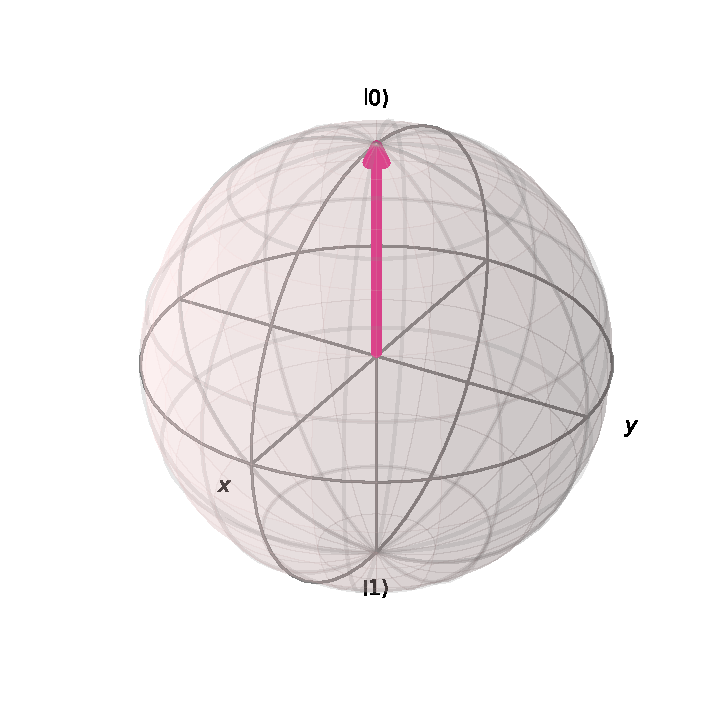
\includegraphics[width=0.95\linewidth]{figures/bloch_0.pdf}
				\caption{$\ket{\psi}=\ket{0}$}
			\end{subfigure}%
			\begin{subfigure}{.35\textwidth}
				\centering
				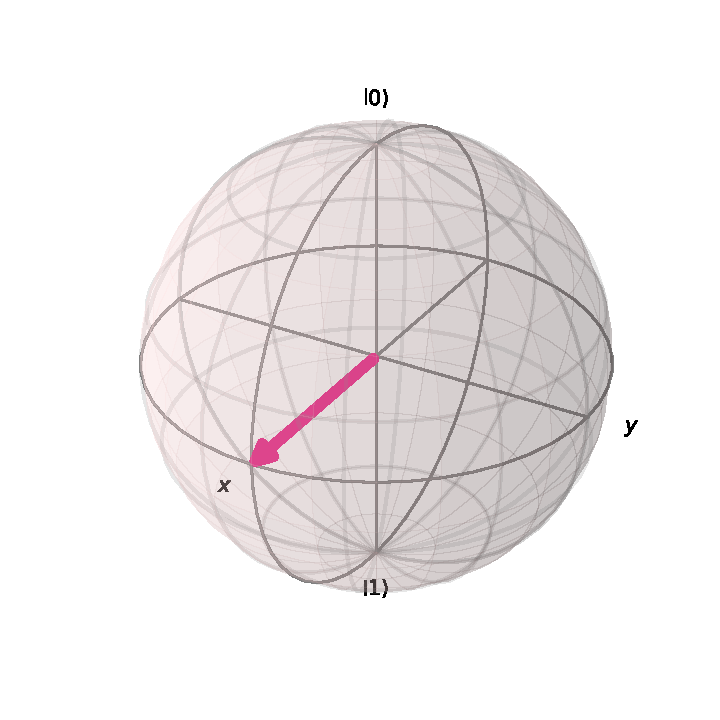
\includegraphics[width=0.95\linewidth]{figures/bloch_superposition.pdf}
				\caption{$\ket{\psi}=\frac{1}{\sqrt{2}}(\ket{0}+\ket{1})$}
			\end{subfigure}
			\caption{Two different qubit states visualized as bloch vectors. (a) has a probability of 100\% to be in the state $\ket{0}$, (b) has a 50\% chance to be either in the state $\ket{0}$ or $\ket{1}$. These visuals were generated using Qiskit \cite{qiskit2024}. The source code for this figure can be found in Listing \ref{lst:bloch_source}}
			\label{fig:bloch_qubits}
		\end{figure}
\section{Entanglement} \label{sec:entanglement}
	With the help of postulate \ref{post:qm_4}, as discussed in section \ref{sec:postulates}, two qubits
	\begin{equation}
		\label{eq:qubit_psi}
		\ket{\psi}=a\ket{0}+b\ket{1}
	\end{equation}
	\begin{equation}
		\label{eq:qubit_phi}
		\ket{\phi}=c\ket{0}+b\ket{1}
	\end{equation}
	can be described together in a composite system by joining their respective Hilbertspaces:
	\begin{equation}
		\label{eq:qubit_composite_hilbertspace}
		\mathcal{H}_{\psi\phi}=\mathcal{H}_\psi\otimes\mathcal{H}_\phi.
	\end{equation}
	Using the notation
	\begin{equation}
		\ket{nm}\equiv\ket{n}\otimes\ket{m},
	\end{equation}
	the computational product basis for this new Hilbertspace is $\{\ket{00},\ket{01},\ket{10},\ket{11}\}$, allowing a state in this Hilbertspace to be in the form of
	\begin{equation}
		\label{eq:allowed_states_in_composite_two_qubits}
		\alpha\ket{00}+\beta\ket{01}+\gamma\ket{10}+\delta\ket{11}.
	\end{equation}
	Postulate \ref{post:qm_4} also states, that the joint state of the two qubits equals to $\ket{\psi}\otimes\ket{\phi}$, which, when considering that both qubits must be normalized, only has two degrees of freedom, while a state prepared in the new Hilbertspace has three degrees of freedom. That means there are states in a composite system, that cannot be realized by only manipulating the qubits on its own. Such a state cannot be seperated into two qubits anymore and is called an entangled state \cite{Nielsen2010-xd}. In this state, the qubits are correlated to each other. The measurement of one qubit determines the measurement outcome of the other qubit. One example of such a preparation would be 
	\begin{equation}
		\label{eq:two_qubit_entangled}
		\ket{\Psi}=\frac{1}{\sqrt{2}}\left(\ket{01}+\ket{10}\right).
	\end{equation}
	For this state, there do not exist two qubit states $\ket{\psi}$ and $\ket{\phi}$ such that $\ket{\psi}\otimes \ket{\phi}=\ket{\Psi}$. Another way of thinking about the state $\ket{\Psi}$ is, that if qubit $\ket{\psi}$ is measured and yields the result $\ket{0}$ the only possible outcome when measuring qubit $\ket{\phi}$ in the same basis is $\ket{1}$. The qubits are dependent on each other.
\chapter{Quantum Circuits} \label{chap:circuits}
Multiple qubits in combination with quantum gates can be arranged to a quantum circuit.
Initially, each qubit is set to the state $\ket{0}$ and subsequently transformed through the application of quantum gates.
Apart from qubits and quantum gates, a quantum circuit also consists of classical bits and measurements.
Qubits can be measured at any point in the circuit.
Upon measurement, the state of a qubit collapses to either $\ket{1}$ or $\ket{0}$, and the result of the measurement is stored in one of the classical bits.
Figure \ref{fig:example_quantum_circuit} shows an example for a simple quantum circuit.
The aim of this chapter is to fully understand and describe this circuit.
\begin{figure}[H]
	\centering
	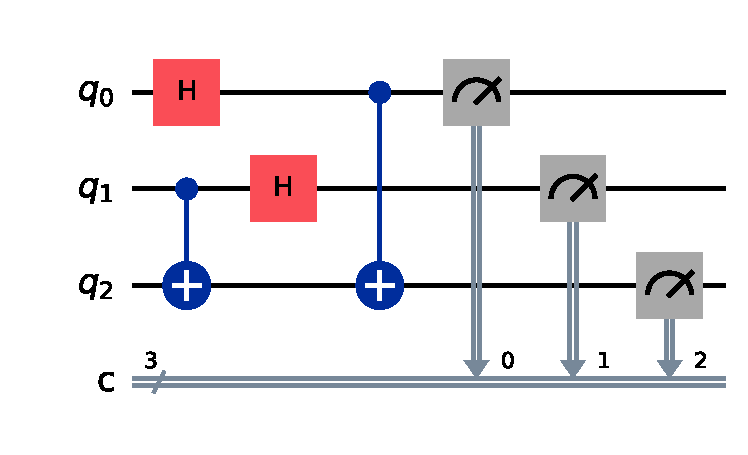
\includegraphics[width=0.5\linewidth]{figures/example_quantum_circuit.pdf}
	\caption{This is an example of a simple quantum circuit. There are three qubits $\{q_0,q_1,q_2\}$, whose states are transformed by two single-qubit gates—Hadamard gates (H) in this case—and two multi-qubit gates, specifically controlled-X (CX) gates. At the end, each qubit is measured, and the result is stored in three classical bits. This visualization of a quantum circuit was generated using Qiskit \cite{qiskit2024}. The source code for this figure can be found in Listing \ref{lst:example_circuit_source}}
	\label{fig:example_quantum_circuit}
\end{figure}
\section{Quantum gates}
	A quantum gate in a quantum circuit can be understood as an Unitary operator that acts either on the state of an individual qubit or on the composite state of multiple qubits.
	\subsection{Single qubit gates}
		As the name implies, a single qubit gate acts on single qubits. Its purpose is to map a state of a qubit into another state,
		therefore it can be described as an Unitary operator
		\begin{equation}
			\label{eq:single_qubit_gate}
			\hat{A}=\alpha\ketbra{0}{0}+\beta\ketbra{1}{0}+\gamma\ketbra{0}{1}+\delta\ketbra{1}{1},
		\end{equation}
		acting on the state $\ket{\psi}=a\ket{0}+b\ket{1}$ of a qubit,
		\begin{equation}
			\label{eq:single_qubit_action}
			\hat{A}\ket{\psi}=(a\alpha+b\gamma)\ket{0} + (a\beta+b\delta)\ket{1}.
		\end{equation}
		The operator $\hat{A}$ can be represented as a $2\times 2$ matrix using the computational basis $\{\ket{0},\ket{1}\}$:
		\begin{equation}
			\label{eq:single_qubit_gate_matrix}
			A^{\{\ket{0},\ket{1}\}}=
			\begin{pmatrix}
				\alpha & \beta  \\
				\gamma & \delta
			\end{pmatrix}
		\end{equation}
		With equation (\ref{eq:single_qubit_action}), gates can be constructed at will for different systems.
		An example is the Hadamard gate $H$, which transforms a qubit in the $\ket{0}$ or $\ket{1}$ state into a state with equal probabilities for $\ket{0}$ and $\ket{1}$ \cite{Rieffel2011-ak}:
		\begin{equation}
			\label{eq:hadamard_condition_1}
			H\ket{0}=\frac{1}{\sqrt{2}}(\ket{0}+\ket{1})
		\end{equation}
		\begin{equation}
			\label{eq:hadamard_condition_2}
			H\ket{1}=\frac{1}{\sqrt{2}}(\ket{0}-\ket{1})
		\end{equation}
		With equations (\ref{eq:hadamard_condition_1}) and (\ref{eq:hadamard_condition_2}) all components $\{\alpha,\beta,\gamma,\delta\}$ of $H$ can be calculated.
		\begin{equation}
			\label{eq:hadamard_matrix}
			H=\frac{1}{\sqrt{2}}
			\begin{pmatrix}
				1 & 1  \\
				1 & -1
			\end{pmatrix}
		\end{equation}
		A more general gate is the $U$ gate. In this gate, three Euler angles \cite{Morin2008-za} are used to rotate the state vector of the qubit.
		\begin{equation}
			\label{eq:u_gate}
			U(\theta,\phi,\lambda) =
			\begin{pmatrix}
				cos\left(\frac{\theta}{2}\right) & -e^{i\lambda}sin\left(\frac{\theta}{2}\right)  \\
				e^{i\phi}sin\left(\frac{\theta}{2}\right) & e^{i(\phi+\lambda)}cos\left(\frac{\theta}{2}\right).
			\end{pmatrix}
		\end{equation}
	\subsection{Multi qubit gates} \label{sec:multi_qubit_gates}
		The real power of quantum circuits lies in manipulating states of qubits based on the state of other qubits.
		This can create entanglement. One example of an entangling gate is the Controlled-NOT ($CNOT$ or $CX$) gate.
		It acts on two qubits where the first qubit acts as a control.
		If the control qubit is in the state $\ket{1}$ it performs the $NOT$ operation on the second qubit. Otherwise the second qubit remains unchanged:
		\begin{equation}
			\label{eq:cx_action_on_eigenstate00}
			CX\ket{00}=\ket{00}
		\end{equation}
		\begin{equation}
			\label{eq:cx_action_on_eigenstate01}
			CX\ket{01}=\ket{01}
		\end{equation}
		\begin{equation}
			\label{eq:cx_action_on_eigenstate10}
			CX\ket{10}=\ket{11}
		\end{equation}
		\begin{equation}
			\label{eq:cx_action_on_eigenstate11}
			CX\ket{11}=\ket{10}
		\end{equation}
		With these conditions, the matrix representation of the $CX$ gate in the computational product basis can be found:
		\begin{equation}
			\label{eq:cx_matrix_representation}
			CX=
			\begin{pmatrix}
				1 & 0 & 0 & 0 \\
				0 & 1 & 0 & 0 \\
				0 & 0 & 0 & 1 \\
				0 & 0 & 1 & 0
			\end{pmatrix}.
		\end{equation}
		Similar to an entangled state vector, as discussed in Section \ref{sec:entanglement}, the controlled-X gate cannot be constructed by the tensorproduct of two single-qubit gates. This can easily be proven by assuming it can be separated into two $2 \times 2$ matrices,
		\begin{equation}
			\label{eq:assume_cx_separable}
			\begin{pmatrix}
				\alpha & \beta \\
				\gamma & \delta
			\end{pmatrix}\otimes
			\begin{pmatrix}
				a & b \\
				c & d
			\end{pmatrix}=
			\begin{pmatrix}
				1 & 0 & 0 & 0 \\
				0 & 1 & 0 & 0 \\
				0 & 0 & 0 & 1 \\
				0 & 0 & 1 & 0
			\end{pmatrix}
		\end{equation}
		leading to a contradiction:
		\begin{equation}
			\label{eq:cx_separability_contradiction}
			\alpha a = \delta c = 1 \Rightarrow \alpha \neq 0 \land c \neq 0 \Rightarrow\!\Leftarrow \alpha c = 0.
		\end{equation}
\section{Circuit calculation} \label{sec:circuit_calculation}
	To calculate the final state of all three qubits in the circuit of Figure \ref{fig:example_quantum_circuit}, the initial state and all gates will be transformed into the three-qubit product basis $\mathcal{B}=\left\{\ket{000},\ket{001},\ket{010},\ket{011},\ket{100},\ket{101},\ket{110},\ket{111}\right\}$. The composite initial state $\ket{\psi_{initial}}$ of the circuit in the basis $\mathcal{B}$ is $\ket{000}$.
	\begin{figure}[H]
		\centering
		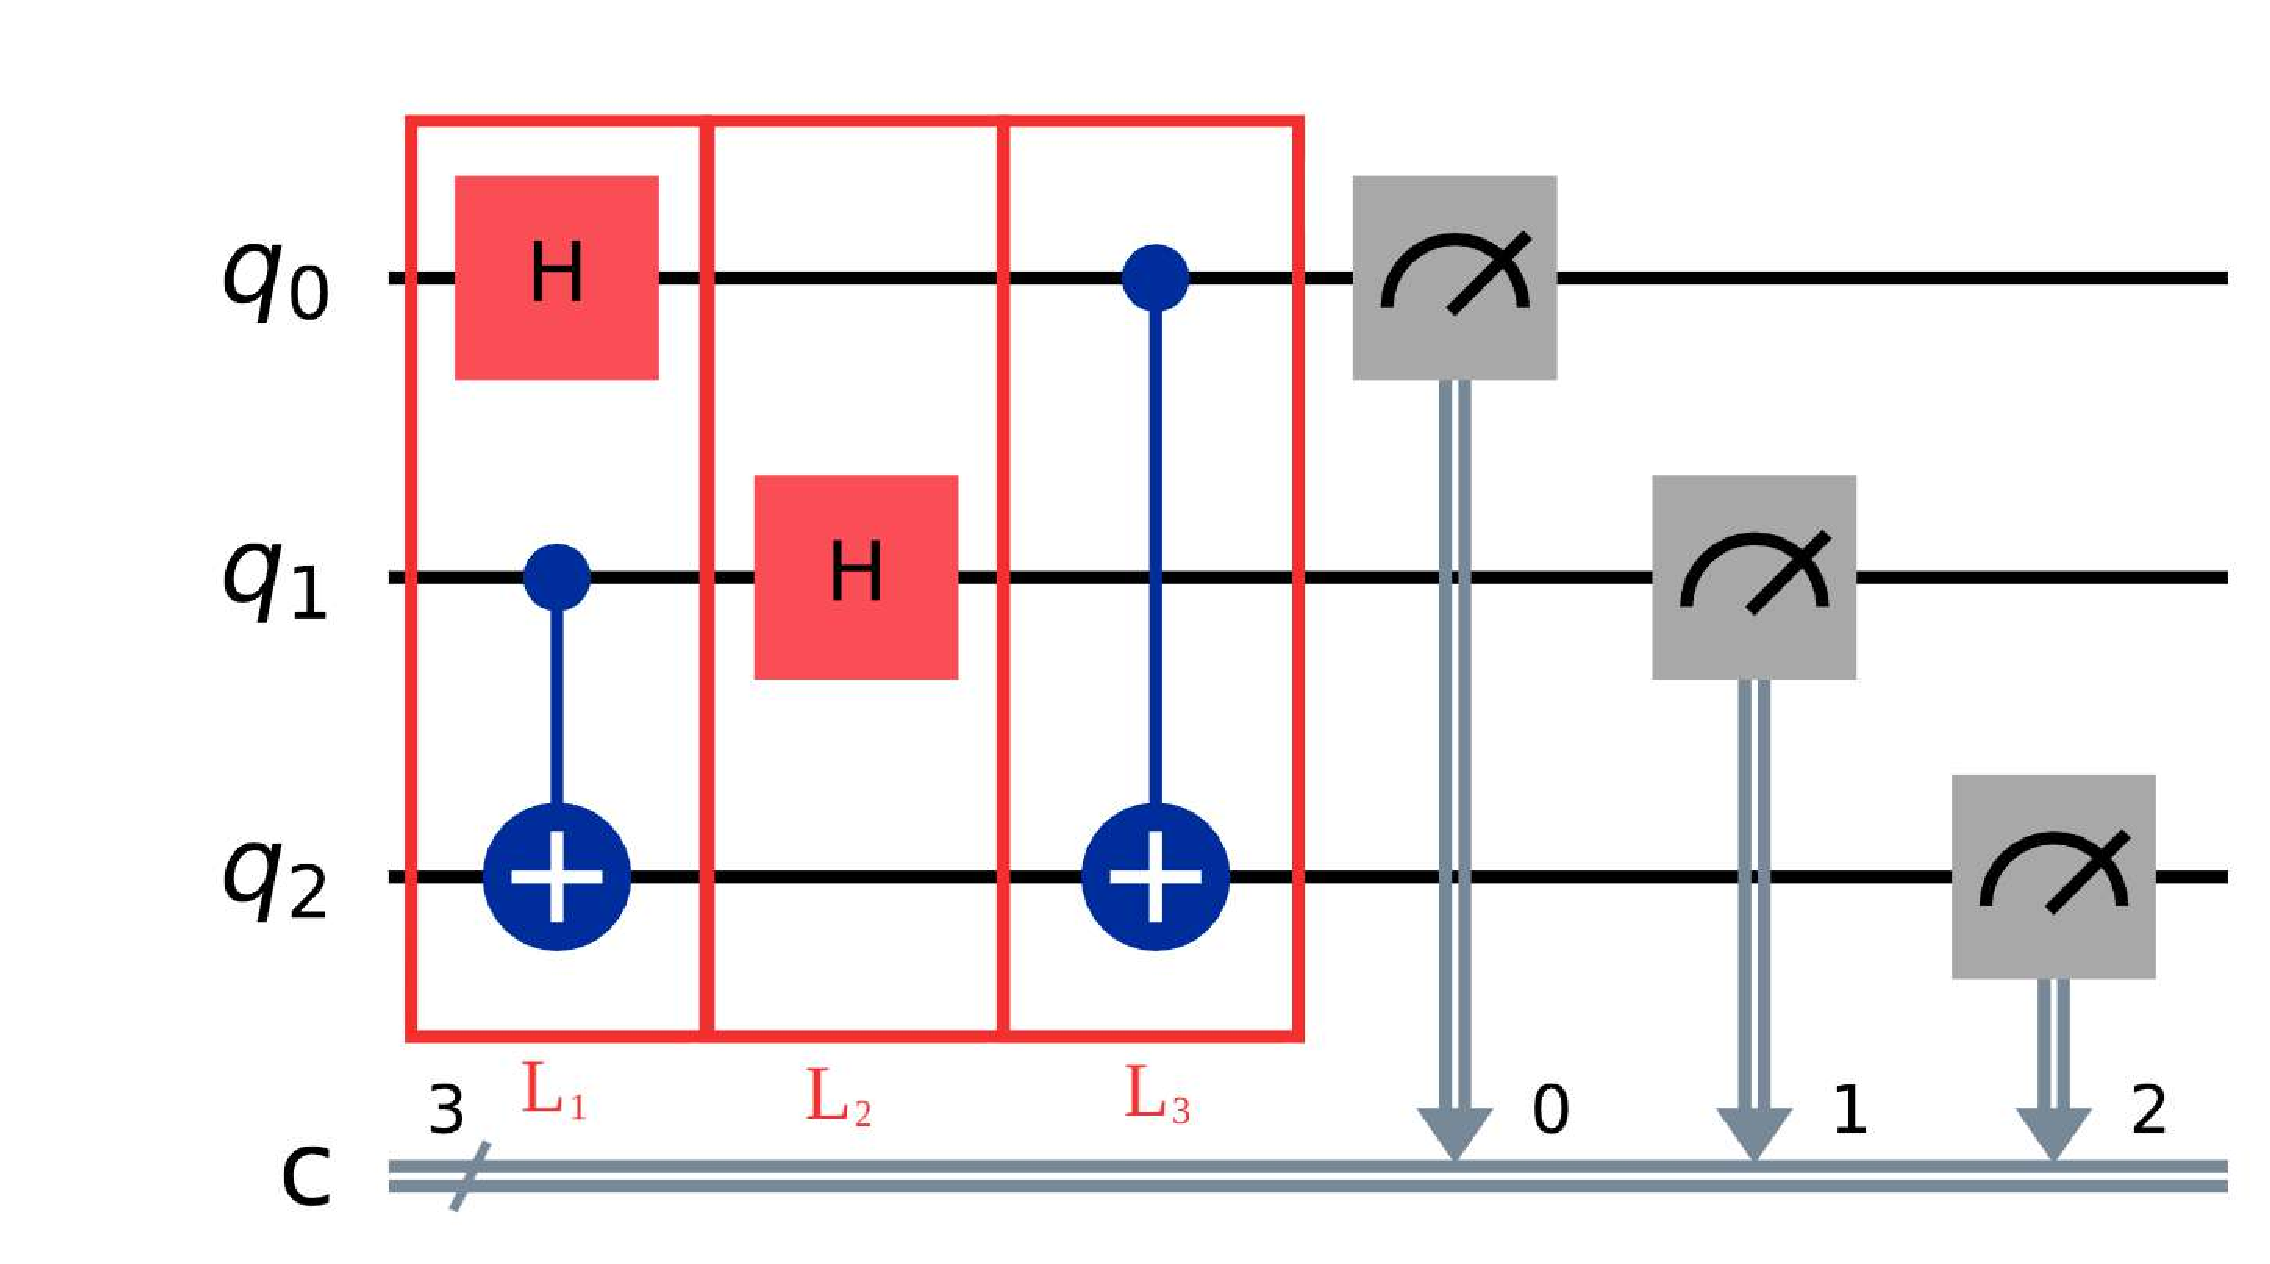
\includegraphics[width=0.5\linewidth]{figures/example_quantum_circuit_with_layers.pdf}
		\caption{The circuit from Figure \ref{fig:example_quantum_circuit} can be split into layers. In every layer, a maximum of one gate act on each qubit.}
		\label{fig:example_quantum_circuit_with_layers}
	\end{figure}
	As shown in Figure \ref{fig:example_quantum_circuit_with_layers}, the circuit can be divided into three layers $L_1$, $L_2$ and $L_3$. Each layer can be imagined as an Unitary operator acting on the composite state of all qubits. The final state $\ket{\psi_{final}}$ can then be determined by applying all operators corresponding to the layers of the circuit to the initial state $\ket{\psi_{initial}}$,
	\begin{equation}
		\label{eq:apply_layers_to_initial_state}
		\ket{\psi_{final}}=\hat{L}_3\hat{L}_2\hat{L}_1\ket{\psi_{initial}}.
	\end{equation}
	To determine the matrix representation of the layers, the matrix representation in the basis $\mathcal{B}$ for each single-qubit gate $U_{(i)}$ and two-qubit gate $U_{(i, j)}$ contained in the layer has to be found. In this notation $i$ and $j$ denote the number of the qubit on which the gate acts, while demanding $i < j$.
	As single-qubit gates leave other qubits untouched, their matrix representation in a basis $\mathcal{B}_N$ for $N$ qubits can be constructed by tensor-products with the identity matrix:
	\begin{equation}
		\label{eq:single_qubit_gate_product_basis}
		U^{\{\mathcal{B}_N\}}_{(i)}=\mathbbm{1}^{\otimes i}\otimes U_{(i)}\otimes \mathbbm{1}^{\otimes N-1-i}
	\end{equation}
	Entangling gates cannot be seperated into single-qubit gates as discussed in Section \ref{sec:multi_qubit_gates}, so to find the matrix representation of entangling gates $U_{(i,j)}$ in the basis $\mathcal{B}_N$ while only knowing the matrix representation of $U_{(i,i+1)}$, a permutation matrix $P$, more specifically a transposition matrix $P_{n\mapsto m}$, has to be applied for entangling gates of non-adjacent qubits that swaps two qubits in a way that qubit $q_i$ and $q_j$ are adjacent,
	\begin{equation}
		\label{eq:qubit_swap}
		q_j\leftrightarrow q_{i+1}
	\end{equation}
	leading to
	\begin{equation}
		\label{eq:two_qubit_gate_product_basis}
		U^{\{\mathcal{B}_N\}}_{(i, j)}=P^{-1}_{i+1\mapsto j}\left(\mathbbm{1}^{\otimes i}\otimes U_{(i,i+1)}\otimes \mathbbm{1}^{\otimes N-2-i}\right)P_{i+1\mapsto j}.
	\end{equation}
	\\
	Coming back to the example from figure \ref{fig:example_quantum_circuit_with_layers} the first layer $L_1$, a Hadamard gate acts on the qubit $q_0$ and a controlled-X gate acts on $q_1$ and $q_2$ where $q_1$ is the control qubit and $q_2$ is the target qubit. Using equations (\ref{eq:single_qubit_gate_product_basis}) and (\ref{eq:two_qubit_gate_product_basis}), $L_1$ can be calculated,
	\begin{equation}
		\label{eq:example_circuit_layer1}
		L_1=\left(H\otimes \mathbbm{1}\otimes \mathbbm{1}\right)\left(\mathbbm{1}\otimes CX\right)=H\otimes CX,
	\end{equation}
	while the permutation matrix $P=\mathbbm{1}$ for $L_1$  as $q_1$ and $q_2$ are already adjacent.
	$L_2$ can be found in a similar fashion as in this layer only a single-qubit Hadamard gate is present:
	\begin{equation}
		\label{eq:example_circuit_layer2}
		L_2=\mathbbm{1}\otimes H\otimes\mathbbm{1}.
	\end{equation}
	In $L_3$ only a controlled-X gate is present. But the qubits it acts on are not adjacent. To make them adjacent a transposition matrix $P_{1\mapsto 2}$ is used. This transposition matrix swaps qubit $q_1$ and $q_2$, so qubit $q_0$ is adjacent to $q_2$. When these qubits are swapped, the basis state order changes. This yields the conditions to determine the permutation matrix:
	\begin{equation}
		\label{eq:example_circuit_permutation_matrix}
		\begin{split}
			P_{1\mapsto 2}\ket{000}&=\ket{000} \\
			P_{1\mapsto 2}\ket{001}&=\ket{010} \\
			P_{1\mapsto 2}\ket{010}&=\ket{001} \\
			P_{1\mapsto 2}\ket{011}&=\ket{011} \\
			P_{1\mapsto 2}\ket{100}&=\ket{100} \\
			P_{1\mapsto 2}\ket{101}&=\ket{110} \\
			P_{1\mapsto 2}\ket{110}&=\ket{101} \\
			P_{1\mapsto 2}\ket{111}&=\ket{111}
		\end{split} \Rightarrow P_{1\mapsto 2}=
		\begin{pmatrix}
			1 & 0 & 0 & 0 & 0 & 0 & 0 & 0 \\
			0 & 0 & 1 & 0 & 0 & 0 & 0 & 0 \\
			0 & 1 & 0 & 0 & 0 & 0 & 0 & 0 \\
			0 & 0 & 0 & 1 & 0 & 0 & 0 & 0 \\
			0 & 0 & 0 & 0 & 1 & 0 & 0 & 0 \\
			0 & 0 & 0 & 0 & 0 & 0 & 1 & 0 \\
			0 & 0 & 0 & 0 & 0 & 1 & 0 & 0 \\
			0 & 0 & 0 & 0 & 0 & 0 & 0 & 1 
		\end{pmatrix}.
	\end{equation}
	$L_3$ can then be determined by using equation (\ref{eq:two_qubit_gate_product_basis}):
	\begin{equation}
		\label{eq:example_circuit_layer3}
		L_3=P^{-1}_{1\mapsto 2}\left(CX\otimes \mathbbm{1}\right)P_{1\mapsto 2}.
	\end{equation}
	Combining all layers yields the circuit Unitary $C$
	\begin{equation}
		\label{eq:example_circuit_unitary}
		C=L_3L_2L_1=\frac{1}{2}
		\begin{pmatrix}
			1 & 1 & 0 & 0 & 1 & 1 & 0 & 0 \\
			0 & 0 & 1 & 1 & 0 & 0 & -1 & -1 \\
			1 & -1 & 0 & 0 & 1 & -1 & 0 & 0 \\
			0 & 0 & -1 & 1 & 0 & 0 & 1 & -1 \\
			0 & 0 & 1 & 1 & 0 & 0 & 1 & 1 \\
			1 & 1 & 0 & 0 & -1 & -1 & 0 & 0 \\
			0 & 0 & -1 & 1 & 0 & 0 & -1 & 1 \\
			1 & -1 & 0 & 0 & -1 & 1 & 0 & 0
		\end{pmatrix}.
	\end{equation}
	By applying $C$ to the initial circuit state $\ket{\psi_{intial}}=\ket{000}$ the final state $\ket{\psi_{final}}$,
	\begin{equation}
		\label{eq:example_circuit_final_state}
		\ket{\psi_{final}}=C\ket{000}=\frac{1}{2}\left(\ket{000}+\ket{010}+\ket{101}+\ket{111}\right)
	\end{equation}
	is computed and the probabilities of measuring each eigenstate can be calculated using equation (\ref{eq:measurement_probability_a}):
	\begin{equation}
		\label{eq:example_circuit_probability_000}
		\abs{\braket{000}{\psi_{final}}}^2=\tfrac{1}{4},
	\end{equation}
	\begin{equation}
		\label{eq:example_circuit_probability_001}
		\abs{\braket{001}{\psi_{final}}}^2=0,
	\end{equation}
	\begin{equation}
		\label{eq:example_circuit_probability_010}
		\abs{\braket{010}{\psi_{final}}}^2=\tfrac{1}{4},
	\end{equation}
	\begin{equation}
		\label{eq:example_circuit_probability_011}
		\abs{\braket{011}{\psi_{final}}}^2=0,
	\end{equation}
	\begin{equation}
		\label{eq:example_circuit_probability_100}
		\abs{\braket{100}{\psi_{final}}}^2=0,
	\end{equation}
	\begin{equation}
		\label{eq:example_circuit_probability_101}
		\abs{\braket{101}{\psi_{final}}}^2=\tfrac{1}{4},
	\end{equation}
	\begin{equation}
		\label{eq:example_circuit_probability_110}
		\abs{\braket{110}{\psi_{final}}}^2=0,
	\end{equation}
	\begin{equation}
		\label{eq:example_circuit_probability_111}
		\abs{\braket{111}{\psi_{final}}}^2=\tfrac{1}{4}.
	\end{equation}
	And indeed, when simulating the circuit with qiskits Aer-Simulator \cite{qiskit2024} with $100000$ runs, the same results are achieved, as seen in Figure \ref{fig:example_circuit_results}.
	\begin{figure}[H]
		\centering
		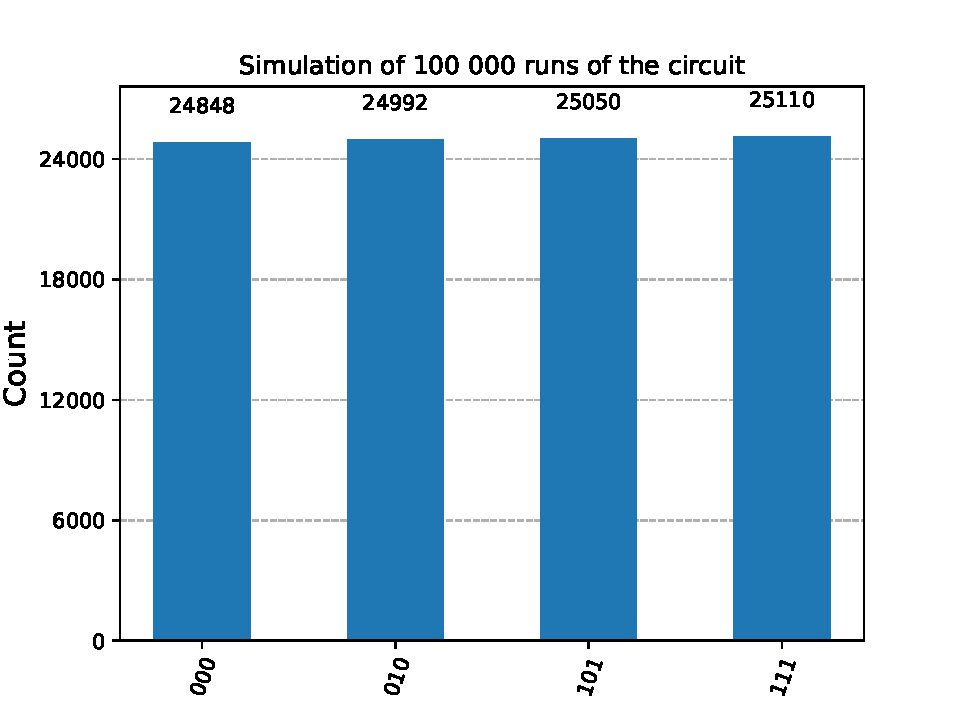
\includegraphics[width=0.7\linewidth]{figures/qc_results.pdf}
		\caption{This plot shows the outcome of a simulation of the circuit from Figure \ref{fig:example_quantum_circuit}. While the states $\ket{000}$, $\ket{010}$, $\ket{101}$ and $\ket{111}$ all have a probability close to $\frac{1}{4}$, the states $\ket{001}$, $\ket{011}$, $\ket{100}$ and $\ket{110}$ are not realized. This coincides with the exact result from equation (\ref{eq:example_circuit_final_state}). This plot was generated using Qiskit \cite{qiskit2024}. The source code for this figure can be found in Listing \ref{lst:circuit_results_source}}
		\label{fig:example_circuit_results}
	\end{figure}

\section{Universal gate sets} \label{sec:universal_gateset}
	The term \textit{Universal Gate Set} is usually defined as follows:
	\begin{definitionbox}
		\textit{A universal gate set is a finite set of gates that can be combined to approximate any Unitary operation on any number of qubits to arbitrary precision.} \cite{Nielsen2010-xd}
	\end{definitionbox}
	It is possible to check if a set of gates is universal by using group-theory methods \cite{Sawicki_2017} or by examining its relation to Unitary t-designs \cite{Sawicki_2022}. One example for a universal gate set that is commonly used is the Clifford + T set \cite{vandaele2024optimal}. It consists of the Hadamard gate $H$ (\ref{eq:hadamard_matrix}), the phase gate $S$ (\ref{eq:s_gate}), the $T$-gate (\ref{eq:t_gate}) and the $CX$ gate (\ref{eq:cx_matrix_representation}). 
	\begin{equation}
		\label{eq:s_gate}
		S=
		\begin{pmatrix}
			1 & 0 \\
			0 & i
		\end{pmatrix}
	\end{equation}
	\begin{equation}
		\label{eq:t_gate}
		T=
		\begin{pmatrix}
			1 & 0 \\
			0 & e^{i\frac{\pi}{4}}
		\end{pmatrix}
	\end{equation}
	By removing the restriction that the set of gates must be finite, the definition becomes simpler:
	\begin{definitionbox}
		\begin{definition}
			\label{def:universal_gate_set}
			A universal gate set is a set of gates that can be combined to produce any Unitary operation on any number of qubits.
		\end{definition}
	\end{definitionbox}
	This definition excludes finite sets of gates, as there are infinetly many Unitary operations. While this definition may not be applicable to real-world scenarios, it is sufficient for this thesis and is therefore used instead of the usual definition.
	One example for a universal gate set that complies with this definition is a set of single-qubit rotations (\ref{eq:u_gate}) in conjunction with the $CZ$-gate,
	\begin{equation}
		\label{eq:cz_gate}
		CZ=
		\begin{pmatrix}
			1 & 0 & 0 & 0 \\
			0 & 1 & 0 & 0 \\
			0 & 0 & 1 & 0 \\
			0 & 0 & 0 & -1 \\
		\end{pmatrix}
	\end{equation}
	Any set of single-qubit gates that is universal for $SU\left(2\right)$, combined with the $CX$-gate (\ref{eq:cx_matrix_representation}) forms a universal gate set \cite{Nielsen2010-xd}. As single-qubit rotations $U\left(\theta,\phi,\lambda\right)$ are universal for $SU\left(2\right)$ by definition and the $CZ$-gate can be constructed using a $CX$ gate and two Hadamard gates,
	\begin{equation}
		\label{eq:cz_construction_with_cx}
		CZ=\left(\mathbbm{1}\otimes H\right)CX\left(\mathbbm{1}\otimes H\right),
	\end{equation}
	the gate set $\{U\left(\theta,\phi,\lambda\right),CZ\}$ is also universal.
	This gate set is later used in this thesis to construct circuits to test circuit compression on.
\chapter{Circuit Compression} \label{chap:compression}
As discussed in Section \ref{sec:multi_qubit_gates}, the workhorse resource for quantum computing is entanglement.
Unfortunately, entanglement also contributes to the fragility of qubits. Entangled qubits in current noisy intermediate-scale quantum (NISQ) devices \cite{Preskill_2018} are extremely sensitive to environmental interactions, causing rapid quantum decoherence \cite{SCHLOSSHAUER20191}, which leads to the degradation of the entangled state \cite{PhysRevLett.93.140404}.
Another problem of NISQ devices is error propagation. Even with little noise, single-qubit errors spreading throughout the quantum circuit can negate any quantum advantage \cite{PRXQuantum.3.040326}. One way to combat these errors are quantum error correction (QEC) algorithms, which can determine whether an error has occured by a suitable measurement and then applying Unitary corrections \cite{QuantumErrorCorrection}. This chapter however investigates another way of mitigating errors -- quantum circuit compression -- by utilizing higher dimensional systems known as \emph{qudits}. By reducing the number of quantum information carriers, the performance of experimental setups can be improved, while simultaneously lowering the resource requirements for quantum error correction through a reduction in entangling-gate count \cite{gao2023role}.
\section{Qudits}
  As discussed in section \ref{sec:particle_in_a_box}, physical systems are not only limited to two states, in fact, most degrees of freedom of physical systems naturally posess more than two eigenstates.
  As qubits are modeled as two-state systems, they lack the capability to utilize higher dimensions, creating the need for a generalization -- the quantum dit (qudit).
  It represents quantum information in a $d$-dimensional Hilbertspace $\mathcal{H}_d$, where $d>2$. For example, a $4$-dimensional qudit (ququart) can be described using a $4$-dimensional hilberstspace $\mathcal{H}_4$ with the computational basis states $\{\ket{0},\ket{1},\ket{2},\ket{3}\}$.
  Such a quqart can be modeled by a composite system of two qubits by encoding the basis states of the quqart onto the composite systems product states $\{\ket{00},\ket{01},\ket{10},\ket{11}\}$ living also on a $4$-dimensional Hilbertspace $\mathcal{H}_4=\mathcal{H}_2\otimes\mathcal{H}_2$. The key difference is, that gates that are capable to entangle qubits, like $CX$ or $CZ$ gates, act locally rather than entangling when applied to a single ququart state:
  \begin{equation}
    \label{eq:quqart_cx_local_gate}
    \begin{split}
      CX\ket{0}&=\ket{0} \\
      CX\ket{1}&=\ket{1} \\
      CX\ket{2}&=\ket{3} \\
      CX\ket{3}&=\ket{2}.
    \end{split}
  \end{equation}
  So by combining qubits to qudits, the amount of entangling operations in a circuit can be reduced, with the limitation being the existence of a real physical system that can accurately represent the qudit.
  \subsection{Qudit Gates}
    When combining $N$ qubits to one qudit it is also critical to understand how arbitrary local qubit gates $U_i$ (\ref{eq:local_qubit_gate_to_qudit_gate}) and entangling qubit gates $U_{i,j}$ (\ref{eq:entangling_qubit_gate_to_qudit_gate}) transform to local qudit gates $U_d$, where $q_i$ and $q_j$ denote qubits being combined, while $i,j \in \{0,1,...,N-1\}$ and $i<j$ and $\mathbbm{1}$ represents the two dimensional identity matrix.

    \begin{equation}
      \label{eq:local_qubit_gate_to_qudit_gate}
      U_d=\mathbbm{1}^{\otimes i}\otimes U_i\otimes\mathbbm{1}^{\otimes N-1-i}
    \end{equation}
    If the entangling qubit gate $U_{i,j}$ acts on qubits which are not adjacent, a transposition matrix $P$ is needed to rearrange the qubits into adjacent positions, as discussed in section \ref{sec:circuit_calculation}, i.e.
    \begin{equation}
      \label{eq:entangling_qubit_gate_to_qudit_gate}
      U_d=P^{-1}_{i+1\mapsto j}\left(\mathbbm{1}^{\otimes i}\otimes U_{i, i+1}\otimes \mathbbm{1}^{\otimes N-2-i}\right)P_{i+1\mapsto j}
    \end{equation}
    To give a better intuition on how qubit-gates transform when merging qubits, it will be demonstrated in the following example.
    \begin{figure}[H]
      \centering
      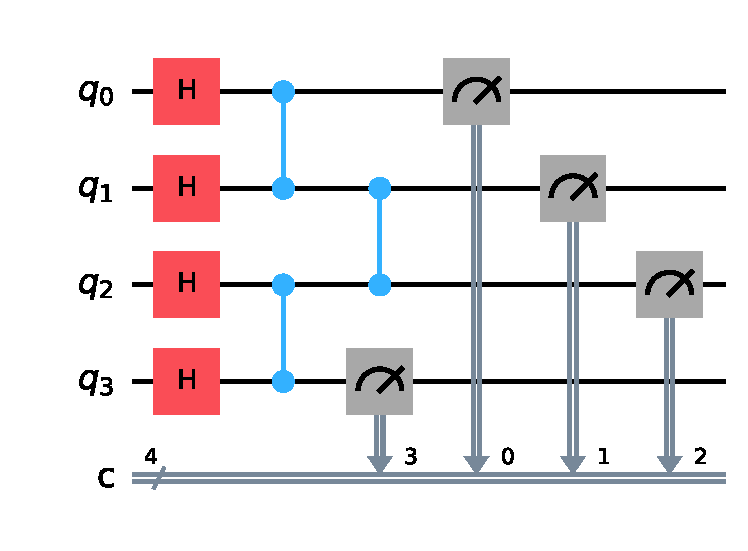
\includegraphics[width=.7\linewidth]{figures/qubit_circuit.pdf}
      \caption{Qubit circuit with four $H$-gates and three $CZ$-gates. This graphic was created using qiskit \cite{qiskit2024}. The source code can be found in Listing \ref{lst:compression_qubit_circuit_source}.}
      \label{fig:compression_qubit_circuit}
    \end{figure}
    In this example, using the circuit from Figure \ref{fig:compression_qubit_circuit}, the qubits $q_0$ and $q_1$ will be merged into a ququart ${q^4}_0$ and the qubits $q_2$ and $q_3$ will be merged into one ququart ${q^4}_1$. There are two ways how to transform local gates. Either they are transformed each into two local $4$-dimensional ququart gates, that act only on a specific level of the ququart, or all gates of one column are combined to one $4$-dimensional ququart gate. In this example, the latter is used. Two $H$-gates transform into a $H_4$-gate:
    \begin{equation}
      \label{eq:4_dimensional_hadamard}
      H_4=H\otimes H=
      \begin{pmatrix}
        1 &  1 &  1 &  1\\
        1 & -1 &  1 & -1\\
        1 &  1 & -1 & -1\\
        1 & -1 & -1 &  1
      \end{pmatrix}
    \end{equation}
    Two of the $CZ$-gates, that are entangling in the qubit circuit become local in the ququart circuit. Their matrix representation does not change. The last $CZ$-gate will still be entangling in the ququart circuit, so it will transform into a $16$-dimensional ququart gate called $CZ_{16}$, its matrix form must be calculated using equation (\ref{eq:entangling_qubit_gate_to_qudit_gate}):
    \begin{equation}
      \label{eq:8_dimensional_cz}
      CZ_{16}=\mathbbm{1}\otimes CZ \otimes\mathbbm{1},
    \end{equation}
    where $\mathbbm{1}$ denote $2$-dimensional identity matrices. The resulting ququarts have four eigenstates, so at least two classical bits are needed to store the measurement results. The resulting ququart circuit is depicted in Figure \ref{fig:compressed_ququart_circuit}.

    \begin{figure}[H]
      \centering
      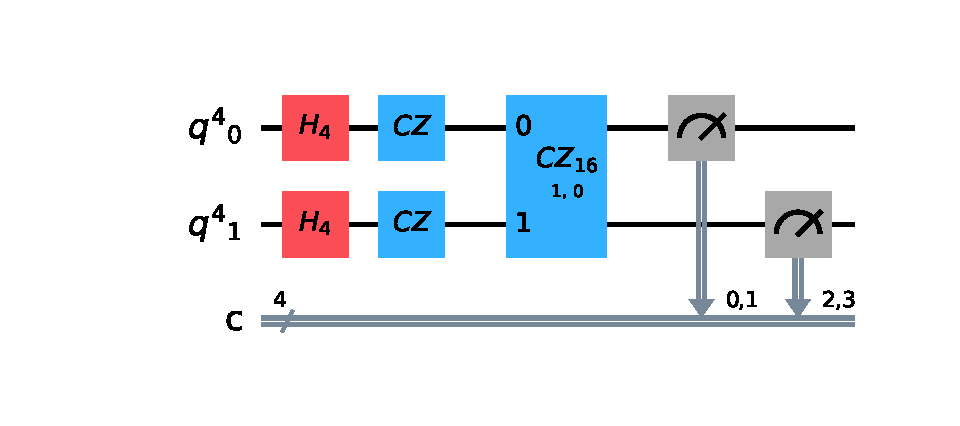
\includegraphics[width=\linewidth]{figures/compressed.pdf}
      \caption{Ququart circuit with two $4$-dimensional $H$-gates denoted by $H_4$, two local $CZ$-gates and one $16$-dimensional entangling $CZ$-gate denoted by $CZ_{16}$. The vertically arranged numbers in the $CZ_{16}$-gate show the numbers of the ququarts it acts on. The horizontally arranged numbers show the internal level of the ququart it acts on. It acts on level $1$ of ququart ${q^4}_0$ (which originated from qubit $q_1$) and on level $0$ of ququart ${q^4}_1$ (from original qubit $q_2$). This graphic was created using qiskit \cite{qiskit2024}. The source code can be found in Listing \ref{lst:compression_ququart_circuit_source}.}
      \label{fig:compressed_ququart_circuit}
    \end{figure}
\section{Algorithm}
  One way to decide what qubits to merge is to create a weighted graph from the circuit and then to cluster nodes of that graph based on their edge-weight with their neighbours \cite{gao2023role}. Using the universal gate set $\{U(\phi,\theta,\lambda), CZ\}$ discussed at the end of section \ref{sec:universal_gateset}, the graph is constructed as follows:
  \begin{enumerate}
    \item From every qubit in the circuit create two graph nodes. The first node represents the state $\ket{0}$ while the second node represents the state $\ket{1}$.
    \item For every local gate $U$ add a graph edge with weight $w_l$ connecting the two nodes that originated from the qubit the gate acts on.
    \item For every entangling gate $CZ$ add a graph edge with weight $w_e$ connecting the second nodes of both qubits it acts on.
  \end{enumerate}
  The $CZ$ gate only affects the $\ket{11}$ state, hence edges are only added to the nodes representing a $\ket{1}$ state. This is also the reason why this algorithm only works for this specific gate set. This simplifies the algorithm, however, it makes it important that $w_l>w_e$ is chosen, otherwise the clustering algorithm may attempt to generate qubits with local $CZ$ gates, which is not possible. A visualization of a graph created from the circuit from Figure \ref{fig:compression_qubit_circuit} is shown in Figure \ref{fig:graph_from_qubit_circuit}.
  \begin{figure}[H]
    \centering
    \includegraphics*[width=.25\textwidth]{figures/graphs/evolution-0/graph_w.pdf}
    \caption{A graph generated from the example circuit from Figure \ref{fig:compression_qubit_circuit} using the algorithm described above with $w_l=4w_e$. The thickness of the edges represent the weights. Nodes connected with a thick line originated from the same qubit, the $H$-gate binds them together. Nodes connected with a thin line are connected through a $CZ$ gate. This graph was visualized using scikit-network \cite{JMLR:v21:20-412}.}
    \label{fig:graph_from_qubit_circuit}
  \end{figure}
  In the next step a graph clustering algorithm groups highly connected nodes together by giving each node a label. In this implementation, any clustering method can be used. The algorithms \textit{Louvain}, \textit{Leiden} and \textit{K-Centers} from scikit-network \cite{JMLR:v21:20-412} are alredy implemented, but other more specialized algorithms, such as for example \textit{gclu} \cite{Sieranoja2021-ik} can easily be added - more on this in section \ref{sec:implementation}.
  \begin{figure}[H]
    \centering
    \scalebox{-1}[1]{\includegraphics*[width=.25\textwidth]{figures/graphs/evolution-0/graph_wl.pdf}}
    \caption{The graph from Figure \ref{fig:graph_from_qubit_circuit} got labeled by the \textit{Louvain} clustering algorithm. Each color represents one label. This graph was visualized using scikit-network \cite{JMLR:v21:20-412}.}
    \label{fig:graph_from_qubit_circuit_labeled}
  \end{figure}
  In Figure \ref{fig:graph_from_qubit_circuit_labeled} the result from labeling the graph from Figure \ref{fig:graph_from_qubit_circuit} is visualized. After labeling, all nodes with the same labels get merged into one new node while preserving edge data in a seperate datastructure, leading to a graph where every node now represents a qubit. Such a graph is visualized in Figure \ref{fig:merged_graph}.
  \begin{figure}[H]
    \centering
    \includegraphics*[width=.25\textwidth]{figures/graphs/evolution-1/graph_w.pdf}
    \caption{This graph is the result of merging every node with the same label from the graph in Figure \ref{fig:graph_from_qubit_circuit_labeled}. Every node now represents a qubit. This graph was visualized using scikit-network \cite{JMLR:v21:20-412}.}
    \label{fig:merged_graph}
  \end{figure}
  This step did not produce a graph representing a qudit circuit but a graph representing a qubit circuit. Therefore, the clustering algorithm is applied again on the new graph, resulting in a ququart circuit graph, shown in Figure \ref{fig:ququart_graph}.
  \begin{figure}[H]
    \centering
    \begin{subfigure}{.25\textwidth}
      \centering
      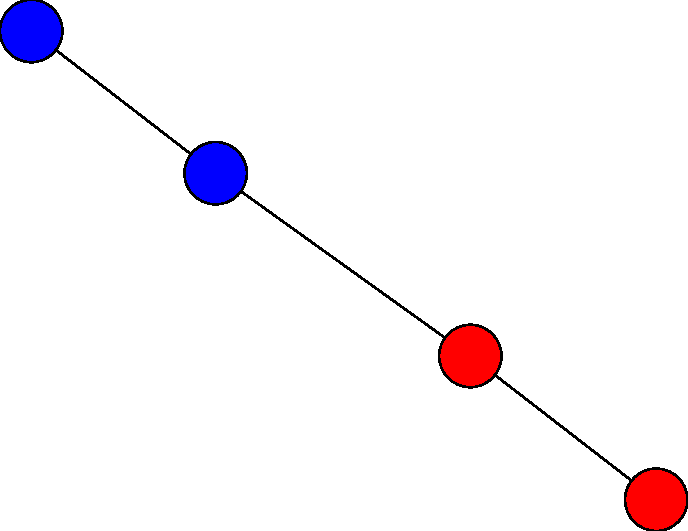
\includegraphics[width=\linewidth]{figures/graphs/evolution-1/graph_wl.pdf}
      \caption{}
    \end{subfigure}%
    \begin{subfigure}{.25\textwidth}
      \centering
      \scalebox{-1}[1]{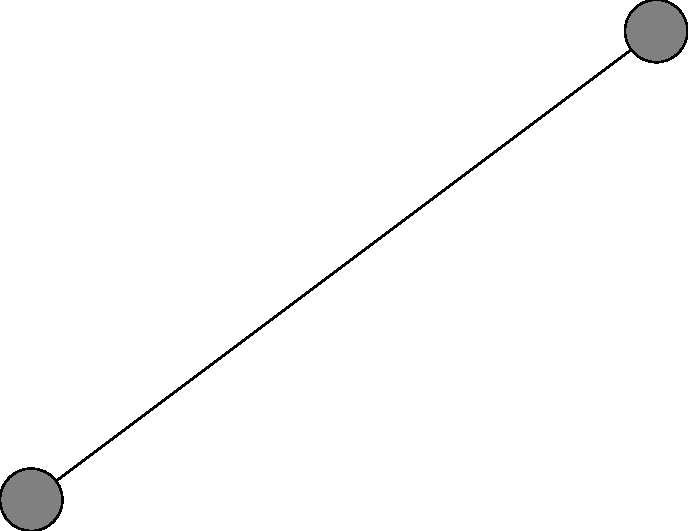
\includegraphics[width=\linewidth]{figures/graphs/evolution-2/graph_w.pdf}}
      \caption{}
    \end{subfigure}
    \caption{The \textit{Louvain} clustering algorithm assigns two labels to the nodes of the graph (a), effectevely merging four qubits into two ququarts. The resulting graph (b) represents exactly the circuit from Figure \ref{fig:compressed_ququart_circuit}. These graphs were visualized using scikit-network \cite{JMLR:v21:20-412}.}
    \label{fig:ququart_graph}
  \end{figure}
  In summary, the algorithm can be described as follows:
  \begin{enumerate}
    \item Create a weighted graph from a circuit
    \item Run a clustering algorithm $c$ that assigns labels to nodes of the graph
    \item Save all gate information from each cluster in a seperate datastructure
    \item Merge all nodes with the same label
    \item Repeat steps 2. to 4. $n$ times
  \end{enumerate}
  where $c$ and $n$ can be chosen depending on the wanted dimension $d$ of the qudit and width of the qubit circuit.
\section{Implementation} \label{sec:implementation}
  The entire source code of the project is publicly available at \url{https://github.com/SimShady/qudit-compression} licensed under the GNU General Public License version 3 \cite{gplv3}. A copy of the source code can also be found in Appendix \ref{sec:project_source}. The project is structured in the following folders and files:
  \begin{itemize}
    \item \texttt{circuits/}
    \begin{itemize}
      \item In this folder, all input circuits are stored in OpenQASM-format \cite{qasm}. Except for the file \texttt{thesis\_circuit\_qiskit\_4.qasm}, every file in this folder is taken from the mqt-qudit-compression project \cite{mato2023compression}.
    \end{itemize}
    \item \texttt{solutions/}
    \begin{itemize}
      \item In this folder, all output circuits and visualizations are stored.
      \item Circuit data is stored in \texttt{solutions/<circuitname>/<algorithmname>/data}
      \item Visuals are stored in \texttt{solutions/<circuitname>/<algorithmname>/visuals}
    \end{itemize}
    \item \texttt{graph.py}
    \item \texttt{circuit.py}
    \item \texttt{clustering.py}
    \item \texttt{processing.py}
    \item \texttt{main.py}
    \item \texttt{circuitinfo.py}
    \item \texttt{requirements.txt}
    \item \texttt{flake.nix}
    \item \texttt{flake.lock}
\end{itemize}
In the following, the source files are described in more detail.
\subsection*{{\Large\texttt{graph.py}} (Listing \ref{lst:graph.py})}
  This file provides a simple datastructure to model a graph using only a list of edges to do so. That means, that if during the clustering process a node loses all edges it is destroyed. That has to be kept in mind when analysing results. Additionaly, an array \texttt{node\_weights} is maintained that keeps track of the size of each node, with the size meaning the number of original nodes it has been merged with. The datastructure has basic methods to create and copy it as well as two special methods \texttt{get\_reduced\_graph\_by\_label} and \texttt{reduce\_graph}.
  \begin{itemize}
    \item \texttt{get\_reduced\_graph\_by\_label} creates a new graph based on provided labels. It is a helper function for \texttt{reduce\_graph}.
    \item \texttt{reduce\_graph} calls the provided clustering algorithm one or more times and creates new graphs while keeping track of the history of graphs and labels used. These history arrays are then returned.
  \end{itemize}
\subsection*{{\Large\texttt{circuit.py}} (Listing \ref{lst:circuit.py})}
  This file contains every datastructure needed to describe a qudit circuit.
  \begin{itemize}
    \item \texttt{Instruction}
    \item \texttt{Qudit}
    \item \texttt{QuditGate}
    \item \texttt{Circuit}
  \end{itemize}
  The \texttt{Instruction} class is just a helper structure that is used to convert qiskit circuits into an instance of \texttt{Circuit}. The classes \texttt{Qudit} and \texttt{QuditGate} are mainly structures to store data about qudits and gates. They have a function to serialize to JSON and some error handling to prevent invalid states. The most important datastructure is the \texttt{Circuit}. It stores a list of qudits and a ordered list of qudit gates, and can be created by passing such two lists to the constructor or from a QASM file. It also has a method to serialize to JSON which calls the serializers of its qudits and gates. The two important methods in this class are:
  \begin{itemize}
    \item \texttt{generate\_weighted\_graph}, which converts the circuit to a weighted graph. The weights $w_l$ and $w_e$ can be chosen. The defaults are $w_l=400$ and $w_e=100$. The implementation of converting a qiskit circuit into a graph was based on the mqt-qudit-compression project \cite{mato2023compression}.
    \item \texttt{get\_updated\_circuit\_by\_labels}, which creates a new circuit based on the current circuit and a set of labels from a graph clustering algorithm.
  \end{itemize}
\subsection*{{\Large\texttt{clustering.py}} (Listing \ref{lst:clustering.py})}
  This file is used as a library for clustering algorithms and also serves as example on how the interface of a clustering function needs to look like to be compatible with this project. A clustering function needs to take a \texttt{Graph} for an argument and return a list of integers representing the labels. The index $i$ of this list denotes the number of the node, while the value at $i$ denotes the label. If additional parameters need to be passed to the underlying clustering function, this can be done using a higher order function demonstrated by the three implemented functions \texttt{louvain}, \texttt{leiden} and \texttt{kcenters}.
\subsection*{{\Large\texttt{processing.py}} (Listing \ref{lst:processing.py}) and {\Large\texttt{main.py}} (Listing \ref{lst:main.py})}
  The file \texttt{processing.py} provides a function that prepares and applies the compression of one circuit using one clustering algorithm. It writes the resulting circuit data and visuals including the history to the \texttt{solutions} folder. The file \texttt{main.py} serves as entrypoint of the program. It looks up all files in the \texttt{circuits} folder and processes each circuit with multiple clustering algorithms using the function from \texttt{processing.py}.
\subsection*{{\Large\texttt{circuitinfo.py}} (Listing \ref{lst:circuitinfo.py})}
  This program serves as utility to inspect generated circuits. For the example circuit from Figure \ref{fig:compressed_ququart_circuit}, it prints: 
  \begin{verbatim}
Number of qudits: 2
Qudit dimensions: [4, 4]
Number of local gates: 6
Number of entangling gates: 1
  \end{verbatim}
  Or for a circuit a little bit more complex (from \texttt{qpeexact\_indep\_qiskit\_31.qasm}):
  \begin{verbatim}
Number of qudits: 7
Qudit dimensions: [38, 4, 4, 4, 4, 4, 4]
Number of local gates: 1408
Number of entangling gates: 571
  \end{verbatim}
\subsection*{Utility files}
  The files \texttt{requirements.txt} (Listing \ref{lst:requirements.txt}), \texttt{flake.nix} (Listing \ref{lst:flake.nix}), \texttt{flake.lock} (Listing \ref{lst:flake.lock}) handle dependency management and support the reproducibility even years after this writing. \texttt{requirements.txt} is used by the python package manager \textit{pip} to install the correct versions of python packages that the project depends on. The other two files are used by Nix \cite{Nix} to create a development shell that replicates the exact environment as it exists at the time of writing. This shell can be activated using the command \texttt{nix-shell}.

\chapter{Conclusion} \label{chap:conclusion}
This thesis explored the concept of quantum circuit compression using higher-dimensional quantum systems (qudits) as an approach to optimizing quantum computations. By leveraging qudits, it is possible to reduce circuit width and the number of entangling gates, which are known to be a major source of noise and decoherence in Noisy Intermediate-Scale Quantum (NISQ) devices. The research focused on the transformation of qubit-based circuits into qudit-based representations and implemented a framework to compress qubit circuits to qudit circuits using clustering algorithms to identify optimal qudit encodings.
\\[12pt]
The results demonstrate that qudit-based architectures can effectively reduce the number of entangling operations while maintaining computational integrity. The proposed algorithm provides a flexible framework for circuit compression and can be extended to support additional optimization techniques. The developed program successfully converts quantum circuits into qudit equivalents, theoretically enabling more efficient execution on quantum hardware that supports higher-dimensional states.
\\[12pt]
Future enhancements to the program could expand support for a broader range of universal gate sets, enabling applications on real quantum hardware. Additionally, refining existing clustering algorithms to incorporate machine learning techniques may further enhance the optimization process. To simplify its adoption in practical use cases, the program could be packaged as a modular software library with well-defined APIs, allowing seamless integration into custom circuit compression applications.
\\[12pt]
By providing a framework for quantum circuit compression, this work contributes to the ongoing effort to improve quantum computing efficiency, paving the way for more scalable and noise-resilient quantum algorithms.

\cleardoublepage
\renewcommand{\chapterpagestyle}{plain_center_pagenumber}
\let\cleardoublepage\clearpage
\appendix
\phantomsection
\addcontentsline{toc}{chapter}{\listfigurename}
\listoffigures
\bibliography{bib/mybib}
\chapter{Appendix}
\section{Figure source code} \label{sec:figure_sourcecode}
  \begin{lstlisting}[language=Python,caption=Source code for Figure \ref{fig:bloch_qubits},label=lst:bloch_source]
 from qiskit import QuantumCircuit
 from qiskit.quantum_info import Statevector
 from qiskit.visualization import plot_bloch_multivector

 qc1 = QuantumCircuit(1)
 qc2 = QuantumCircuit(1)
 qc2.h(0)

 state1 = Statevector(qc1)*1.03
 state2 = Statevector(qc2)*1.03
 fig1 = plot_bloch_multivector(state1)
 fig1.get_axes()[0].set_title("")
 fig2 = plot_bloch_multivector(state2)
 fig2.get_axes()[0].set_title("")

 fig1.savefig("bloch_0.pdf")
 fig2.savefig("bloch_superposition.pdf")
  \end{lstlisting}
  \begin{lstlisting}[language=Python,caption=Source code for Figure \ref{fig:example_quantum_circuit},label=lst:example_circuit_source]
 from qiskit import QuantumCircuit
 from qiskit.circuit import QuantumRegister, ClassicalRegister

 qr = QuantumRegister(3, name="q")
 cr = ClassicalRegister(3, name="c")
 qc = QuantumCircuit(qr, cr)

 q0,q1,q2 = qr
 c0,c1,c2 = cr

 qc.h(q0)
 qc.cx(q1,q2)
 qc.h(q1)
 qc.cx(q0, q2)
 qc.measure(q0, c0)
 qc.measure(q1, c1)
 qc.measure(q2, c2)

 qc.draw(output="mpl", filename="example_quantum_circuit.pdf")
  \end{lstlisting}
  \begin{lstlisting}[language=Python,caption=Source code for Figure \ref{fig:example_circuit_results},label=lst:circuit_results_source]
 from qiskit import QuantumCircuit, transpile
 from qiskit.circuit import QuantumRegister, ClassicalRegister
 from qiskit_aer import AerSimulator
 from qiskit.visualization import plot_histogram

 qr = QuantumRegister(3, name="q")
 cr = ClassicalRegister(3, name="c")
 qc = QuantumCircuit(qr, cr)

 q0,q1,q2 = qr
 c0,c1,c2 = cr

 qc.h(q0)
 qc.cx(q1,q2)
 qc.h(q1)
 qc.cx(q0, q2)
 qc.measure(q0, c0)
 qc.measure(q1, c1)
 qc.measure(q2, c2)

 simulator = AerSimulator()
 circ = transpile(qc, simulator)

 result = simulator.run(qc, shots=100000).result()
 counts = result.get_counts(qc)
 plot_histogram(
   counts,
   title="Simulation of 100 000 runs of the circuit",
   filename="qc_results.pdf"
 )
  \end{lstlisting}
  \begin{lstlisting}[language=Python,caption=Source code fore Figure \ref{fig:compression_qubit_circuit},label=lst:compression_qubit_circuit_source]
 from qiskit import QuantumCircuit

 qc = QuantumCircuit(4,4)
 qc.h(0)
 qc.h(1)
 qc.h(2)
 qc.h(3)
 qc.cz(0,1)
 qc.cz(2,3)
 qc.cz(1,2)
 qc.measure(0,0)
 qc.measure(1,1)
 qc.measure(2,2)
 qc.measure(3,3)

 qc.draw(output="mpl", filename="qubit_circuit.pdf")
  \end{lstlisting}
  \begin{lstlisting}[language=Python,caption=Source code fore Figure \ref{fig:compressed_ququart_circuit},label=lst:compression_ququart_circuit_source]
 from matplotlib.figure import Figure
 from qiskit import ClassicalRegister, QuantumCircuit, QuantumRegister
 from qiskit.circuit import Gate

 qr = QuantumRegister(2, name='q^4')
 cr = ClassicalRegister(4, name='c')
 qc = QuantumCircuit(qr,cr)
 qc.append(Gate(name=r'$H_4$', num_qubits=1, params=[]),[0])
 qc.append(Gate(name=r'$H_4$', num_qubits=1, params=[]),[1])
 qc.append(Gate(name=r'$CZ$', num_qubits=1, params=[]),[0])
 qc.append(Gate(name=r'$CZ$', num_qubits=1, params=[]),[1])
 qc.append(Gate(name=r'$CZ_{16}$', num_qubits=2, params=[1,0]),[0,1])
 qc.measure(0,0)
 qc.measure(1,2)

 fig: Figure = qc.draw(output="mpl", style={
   'displaycolor': {
     '$H_4$': ('#fA4D56', '#000000'),
     '$CZ$': ('#33B1FF', '#000000'),
     '$CZ_{16}$': ('#33B1FF', '#000000')
   }
 }) # type: ignore
 ax = fig.get_axes()[0]
 ax.text(
     2.77608 + 1.6,
     -2 + 0.1,
     ",1",
     ha="left",
     va="bottom",
     fontsize=0.8 * 13,
     color="#000000",
     clip_on=True,
     zorder=13,
 )
 ax.text(
     3.77608 + 1.6,
     -2 + 0.1,
     ",3",
     ha="left",
     va="bottom",
     fontsize=0.8 * 13,
     color="#000000",
     clip_on=True,
     zorder=13,
 )
 fig.savefig("compressed.pdf")
  \end{lstlisting}
\section{Project source code} \label{sec:project_source}
  \begin{lstlisting}[language=Python,caption=\texttt{graph.py},label=lst:graph.py]
from typing import Callable

class Graph:
  def __init__(
    self,
    edge_list: list[tuple[int, int, int]],
    node_weights: list[int]
  ):
    self.edge_list = edge_list.copy()
    self.node_weights = node_weights.copy()
  
  def get_reduced_graph_by_label(
    self,
    labels: list[int]
  ) -> "Graph":
    new_node_weights = [0]*len(set(labels))
    for i in range(len(labels)):
      label = labels[i]
      new_node_weights[label] += self.node_weights[i]

    new_edge_list = []
    for edge in self.edge_list:
      node1 = edge[0]
      node2 = edge[1]
      weight = edge[2]
      if labels[node1] != labels[node2]:
        new_edge_list.append((labels[node1], labels[node2], weight))
    return Graph(new_edge_list, new_node_weights)
  
  def reduce_graph(
    self,
    clustering_function: Callable[["Graph"],list[int]],
    max_runs=1
  ) -> tuple[list["Graph"], list[list[int]]]:
    graph_history: list["Graph"] = []
    labels_history = []
    graph = self.copy()

    graph_history.append(graph)
    for runs in range(max_runs):
      labels = clustering_function(graph)
      graph = graph.get_reduced_graph_by_label(labels)
      if not graph.edge_list:
        break # stop if reduced graph does not have any edges left
      labels_history.append(labels)
      graph_history.append(graph.copy())
    return graph_history, labels_history
  
  def copy(self) -> "Graph":
    return Graph(self.edge_list.copy(), self.node_weights.copy())
  \end{lstlisting}
  \begin{lstlisting}[language=Python,caption=\texttt{circuit.py},label=lst:circuit.py]
import math
import json
from qiskit import QuantumCircuit

from graph import Graph

class Instruction:
  def __init__(
    self, name: str,
    qubits: list[int],
    params: list[float]
  ):
    self.name = name
    self.qubits = qubits.copy()
    self.params = params.copy()

class Qudit:
  def __init__(
    self, number: int,
    dimensions: int
  ):
    self.number = number
    self.dimensions = dimensions
  
  def toJSON(self) -> str:
    return json.dumps({
      "number": self.number,
      "dimensions": self.dimensions
    })

  def has_level(self, level: int) -> bool:
    return level >=0 and level < self.dimensions

class QuditGate:
  def __init__(
    self, name: str,
    qudits: list[Qudit],
    levels: list[int],
    euler_angles: tuple[float, float, float]=(0, 0, 0)
  ):
    self.name = name
    self.qudits = qudits
    self.euler_angles = euler_angles
    for i in range(len(self.qudits)):
      qudit = self.qudits[i]
      level = levels[i]
      if (not qudit.has_level(levels[i])):
        raise ValueError(
          f"Qudit {qudit.number} has dimension {qudit.dimensions}, it has no level {level}"
        )
    self.levels = levels

  def toJSON(self) -> str:
    return json.dumps({
      "name": self.name,
      "qudits": [qudit.number for qudit in self.qudits],
      "levels": self.levels,
      "euler_angles": self.euler_angles
    })

class Circuit:
  def __init__(
    self, qudits: list[Qudit],
    gate_list: list[QuditGate]
  ):
    self.qudits = qudits
    self.gate_list = gate_list

  def toJSON(self) -> str:
    return json.dumps({
      "qudits": [json.loads(qudit.toJSON()) for qudit in self.qudits],
      "gates": [json.loads(gate.toJSON()) for gate in self.gate_list]
    })
  
  @staticmethod
  def from_qasm(file: str) -> "Circuit":
    qc = QuantumCircuit.from_qasm_file(file)
    instructions, num_qubits = Circuit.__collect_instructions(qc)
    qudits: list[Qudit] = [Qudit(i, 1) for i in range(num_qubits*2)]
    gate_list: list[QuditGate] = []
    for instruction in instructions:
      if instruction.name != "measure" and instruction.name != "barrier":
        if instruction.name == "cz":
          control_qubit = instruction.qubits[0]
          target_qubit = instruction.qubits[1]
          control_qudit = qudits[control_qubit*2+1] # qubit level 1
          target_qudit = qudits[target_qubit*2+1] # qubit level 1
          gate = QuditGate("cz", [control_qudit, target_qudit], [0, 0])
          gate_list.append(gate)
        else:
          qubit = instruction.qubits[0]
          gate_qudits = [qudits[qubit*2], qudits[qubit*2+1]]
          euler_angles: tuple[float, float, float] = (0, 0, 0)
          match instruction.name:
            case "u1":
              euler_angles = (0, 0, instruction.params[0])
            case "u2":
              euler_angles = (math.pi/2, instruction.params[1], instruction.params[0])
            case "u3":
              euler_angles = (instruction.params[2], instruction.params[1], instruction.params[0])
            case _:
              raise ValueError("Unsupported gate " + instruction.name)
          gate = QuditGate("u", gate_qudits, [0, 0], euler_angles)
          gate_list.append(gate)
    return Circuit(qudits, gate_list)
  
  def generate_weighted_graph(self, local_weight=400, entangling_weight=100) -> Graph:
    edge_list: list[tuple[int, int, int]] = []
    for gate in self.gate_list:
      edge_list.append((gate.qudits[0].number, gate.qudits[1].number, entangling_weight if gate.name == "cz" else local_weight))
    qudit_dimensions = [qudit.dimensions for qudit in self.qudits]
    return Graph(edge_list, node_weights=qudit_dimensions)
  
  def get_updated_circuit_by_labels(self, labels: list[int]) -> "Circuit":
    if (len(labels) != len(self.qudits)):
      raise ValueError("Every qudit needs a label")
    
    qudits = [Qudit(i, 0) for i in range(len(set(labels)))]
    for i, label in enumerate(labels):
      qudits[label].dimensions += self.qudits[i].dimensions
    
    new_gate_list: list[QuditGate] = []

    for gate in self.gate_list:
      gate_qudits: list[Qudit] = []
      gate_qudit_levels: list[int] = []
      first_level = (gate.qudits[0].number, gate.levels[0])
      second_level = (gate.qudits[-1].number, gate.levels[-1])
      first_compressed_level = self.__get_compressed_qudit_level(labels, first_level)
      second_compressed_level = self.__get_compressed_qudit_level(labels, second_level)
      gate_qudits.append(qudits[first_compressed_level[0]])
      if first_compressed_level[0] != second_compressed_level[0]:
        gate_qudits.append(qudits[second_compressed_level[0]])
      gate_qudit_levels.append(first_compressed_level[1])
      gate_qudit_levels.append(second_compressed_level[1])
      new_gate = QuditGate(gate.name, gate_qudits, gate_qudit_levels, gate.euler_angles)
      new_gate_list.append(new_gate)
    return Circuit(qudits, new_gate_list)   

  def __get_compressed_qudit_level(self, labels: list[int], qudit_level: tuple[int, int]) -> tuple[int, int]:
    grouped_labels: list[list[int]] = [[] for i in range(len(set(labels)))]
    for i in range(len(labels)):
      grouped_labels[labels[i]].append(i)
    
    original_qudits = [(qudit.number, qudit.dimensions) for qudit in self.qudits]
    
    original_qudit_idx, level_within_qudit = qudit_level

    for compressed_idx, label in enumerate(grouped_labels):
      if original_qudit_idx in label:
        offset = sum(original_qudits[i][1] for i in label if i < original_qudit_idx)
        new_level_within_compressed = offset + level_within_qudit
        return (compressed_idx, new_level_within_compressed)
    
    raise ValueError("No possible qudit level found")
    
  
  @staticmethod
  def __collect_instructions(qc: QuantumCircuit) -> tuple[list[Instruction], int]:
    num_qubits = len(qc.qubits)
    register_offset_mapper = {}
    last_offset = 0

    for register in qc.qregs:
      register_offset_mapper[register.name] = last_offset
      last_offset = last_offset + register.size

    instructions: list[Instruction] = []
    for _i, gate in enumerate(qc.data):
      name = ""
      qubits: list[int] = []
      params: list[float] = []

      for field in gate:
        if "library" in str(field) or "circuit" in str(field) or "Instruction" in str(field):
          name = field.name
          params = field.params

        if "QuantumRegister" in str(field):
          qubits += [(register_offset_mapper[f._register.name] + f._index) for f in field]

      instructions.append(Instruction(name, qubits, params))

    return instructions, num_qubits
  \end{lstlisting}
  \begin{lstlisting}[language=Python,caption=\texttt{clustering.py},label=lst:clustering.py]
from sknetwork.clustering import Louvain, Leiden, KCenters
from sknetwork.data.parse import from_edge_list

from graph import Graph
from typing import Callable

def louvain(modularity="dugue")-> Callable[[Graph], list[int]]:
  def clustering_function(graph: Graph) -> list[int]:
    louvain = Louvain(modularity=modularity)
    adjacency = from_edge_list(graph.edge_list, weighted=True)
    return louvain.fit_predict(adjacency) # type: ignore
  return clustering_function

def leiden(modularity="dugue") -> Callable[[Graph], list[int]]:
  def clustering_function(graph: Graph) -> list[int]:
    leiden = Leiden(modularity=modularity)
    adjacency = from_edge_list(graph.edge_list, weighted=True)
    return leiden.fit_predict(adjacency) # type: ignore
  return clustering_function

def kcenters(mean_cluster_size: int) -> Callable[[Graph], list[int]]:
  def clustering_function(graph: Graph) -> list[int]:
    kcenters = KCenters(n_clusters = len(graph.node_weights) // mean_cluster_size)
    adjacency = from_edge_list(graph.edge_list, weighted=True)
    return kcenters.fit_predict(adjacency) # type: ignore
  return clustering_function
  \end{lstlisting}
  \begin{lstlisting}[language=Python,caption=\texttt{processing.py},label=lst:processing.py]
from os import makedirs
from os.path import join, exists
from typing import Callable
from sknetwork.visualization import visualize_graph
from sknetwork.data.parse import from_edge_list
from circuit import Circuit
from graph import Graph

def process_circuit(circuit_file: str, out_dir: str, clustering_function: Callable[[Graph], list[int]], max_runs=1) -> int:
  circuit = Circuit.from_qasm(circuit_file)
  graph = circuit.generate_weighted_graph()
  graph_history, labels_history = graph.reduce_graph(clustering_function, max_runs=max_runs)

  for evolution in range(len(graph_history)):
    evolution_dirname = "evolution-" + str(evolution)
    visual_dir = join(out_dir, "visuals", evolution_dirname)
    data_dir = join(out_dir, "data", evolution_dirname)
    if not exists(visual_dir):
      makedirs(visual_dir)
    if not exists(data_dir):
      makedirs(data_dir)

    # save data
    with open(join(data_dir, "circuit.json"), "w+") as data_file:
      data_file.write(circuit.toJSON())

    # generate svg
    sknetwork_graph = from_edge_list(graph_history[evolution].edge_list, weighted=True)
    visualize_graph(sknetwork_graph, filename=join(visual_dir, "graph"), node_size=20) # type: ignore
    visualize_graph(sknetwork_graph, filename=join(visual_dir, "graph_w"), node_size=20, display_edge_weight=True) # type: ignore

    if (evolution < len(labels_history)): # Last graph has no labels
      circuit = circuit.get_updated_circuit_by_labels(labels_history[evolution])
      visualize_graph(sknetwork_graph, filename=join(visual_dir, "graph_l"), node_size=20, labels=labels_history[evolution]) # type: ignore
      visualize_graph(sknetwork_graph, filename=join(visual_dir, "graph_wl"), node_size=20, labels=labels_history[evolution], display_edge_weight=True) # type: ignore
  return len(labels_history) # return actual runs
  \end{lstlisting}
  \begin{lstlisting}[language=Python,caption=\texttt{main.py},label=lst:main.py]
from os import listdir
from os.path import isfile, join
from processing import process_circuit

import clustering

circuits_dir = "circuits"
solutions_dir = "solutions"

circuit_files = [f for f in listdir(circuits_dir) if isfile(join(circuits_dir, f))]

for circuit_file in circuit_files:
  out_dir = join(solutions_dir, circuit_file[:-5])
  runs = process_circuit(join(circuits_dir, circuit_file), join(out_dir, "louvain"), clustering.louvain(modularity="dugue"), max_runs=2)
  print("processed file '%s' with algorithm louvain (dugue) in %d runs" % (circuit_file, runs))
  runs = process_circuit(join(circuits_dir, circuit_file), join(out_dir, "leiden"), clustering.leiden(modularity="dugue"), max_runs=2)
  print("processed file '%s' with algorithm leiden (dugue) in %d runs" % (circuit_file, runs))
  runs = process_circuit(join(circuits_dir, circuit_file), join(out_dir, "kcenters"), clustering.kcenters(mean_cluster_size=4))
  print("processed file '%s' with algorithm kcenters (mean_cluster_size 4) in %d runs" % (circuit_file, runs))
  \end{lstlisting}
  \begin{lstlisting}[caption=\texttt{requirements.txt},label=lst:requirements.txt]
contourpy==1.3.0
cycler==0.12.1
dill==0.3.8
fonttools==4.53.1
kiwisolver==1.4.5
matplotlib==3.9.2
mpmath==1.3.0
numpy==1.26.4
packaging==24.1
pbr==6.1.0
pillow==10.4.0
pylatexenc==2.10
pyparsing==3.1.4
python-dateutil==2.9.0.post0
qiskit==1.2.0
rustworkx==0.15.1
scikit-network==0.33.0
scipy==1.14.1
six==1.16.0
stevedore==5.3.0
symengine==0.11.0
sympy==1.13.2
typing_extensions==4.12.2    
  \end{lstlisting}
  \begin{lstlisting}[language=Python,caption=\texttt{circuitinfo.py},label=lst:circuitinfo.py]
import sys
import json

def help():
  print("Usage: python circuitinfo.py path/to/circuit.json")

file = sys.argv[1]

if (len(sys.argv) < 2):
  help()
else:
  filename = sys.argv[1]
  try:
    with open(filename, 'r', encoding='utf-8') as file:
      data = json.load(file)
      qudits = data["qudits"]
      dimensions = [qudit["dimensions"] for qudit in qudits]
      local_gates = 0
      entangling_gates = 0
      for gate in data["gates"]:
        if len(gate["qudits"]) > 1:
          entangling_gates += 1
        else:
          local_gates += 1
      print("Number of qudits:", len(qudits))
      print("Qudit dimensions:", dimensions)
      print("Number of local gates:", local_gates)
      print("Number of entangling gates:", entangling_gates)
  except FileNotFoundError:
    print(f"Error: The file '{filename}' was not found.")
  \end{lstlisting}
  \begin{lstlisting}[language=Nix,caption=\texttt{flake.nix},label=lst:flake.nix]
{
  description = "qudit-compression";
  inputs.nixpkgs.url = "github:NixOS/nixpkgs/nixos-unstable";
  inputs.flake-utils.url = "github:numtide/flake-utils";

  outputs = { self, nixpkgs, flake-utils }:
    flake-utils.lib.eachDefaultSystem (system: let
      pkgs = nixpkgs.legacyPackages.${system};
      lib = nixpkgs.lib;
      pythonldlibpath = lib.makeLibraryPath (with pkgs; [
        zlib
        zstd
        stdenv.cc.cc
        curl
        openssl
        attr
        libssh
        bzip2
        libxml2
        acl
        libsodium
        util-linux
        xz
        systemd
      ]);
    in {
      devShell = pkgs.mkShell {
        nativeBuildInputs = [ pkgs.bashInteractive ];
        buildInputs = with pkgs; [
          python311
        ];
        shellHook = with pkgs; ''
          ${python311}/bin/python -m venv ./.virtualenv
          source ./.virtualenv/bin/activate
          export LD_LIBRARY_PATH="${pythonldlibpath}"
          pip install -r requirements.txt
        '';
      };
    });
}
  \end{lstlisting}
  \begin{lstlisting}[caption=\texttt{flake.lock},label=lst:flake.lock]
{
  "nodes": {
    "flake-utils": {
      "inputs": {
        "systems": "systems"
      },
      "locked": {
        "lastModified": 1731533236,
        "narHash": "sha256-l0KFg5HjrsfsO/JpG+r7fRrqm12kzFHyUHqHCVpMMbI=",
        "owner": "numtide",
        "repo": "flake-utils",
        "rev": "11707dc2f618dd54ca8739b309ec4fc024de578b",
        "type": "github"
      },
      "original": {
        "owner": "numtide",
        "repo": "flake-utils",
        "type": "github"
      }
    },
    "nixpkgs": {
      "locked": {
        "lastModified": 1734119587,
        "narHash": "sha256-AKU6qqskl0yf2+JdRdD0cfxX4b9x3KKV5RqA6wijmPM=",
        "owner": "NixOS",
        "repo": "nixpkgs",
        "rev": "3566ab7246670a43abd2ffa913cc62dad9cdf7d5",
        "type": "github"
      },
      "original": {
        "owner": "NixOS",
        "ref": "nixos-unstable",
        "repo": "nixpkgs",
        "type": "github"
      }
    },
    "root": {
      "inputs": {
        "flake-utils": "flake-utils",
        "nixpkgs": "nixpkgs"
      }
    },
    "systems": {
      "locked": {
        "lastModified": 1681028828,
        "narHash": "sha256-Vy1rq5AaRuLzOxct8nz4T6wlgyUR7zLU309k9mBC768=",
        "owner": "nix-systems",
        "repo": "default",
        "rev": "da67096a3b9bf56a91d16901293e51ba5b49a27e",
        "type": "github"
      },
      "original": {
        "owner": "nix-systems",
        "repo": "default",
        "type": "github"
      }
    }
  },
  "root": "root",
  "version": 7
}    
  \end{lstlisting}
\end{document}